% Created 2026-02-25 Wed 01:20
% Intended LaTeX compiler: lualatex
\documentclass[a4paper, 11pt]{article}
\usepackage{amsmath}
\usepackage{amssymb}
\usepackage{fontspec}
\setmonofont{Menlo}[Scale=0.9]
\usepackage{graphicx}
\usepackage{longtable}
\usepackage{wrapfig}
\usepackage{rotating}
\usepackage[normalem]{ulem}
\usepackage{capt-of}
\usepackage[dvipsnames]{xcolor}
\usepackage{hyperref}

% Paragraph heading formatting (for deep headline levels)
\usepackage{titlesec}
\titleformat{\paragraph}{\normalfont\normalsize\bfseries}{\theparagraph}{1em}{}
\titlespacing*{\paragraph}{0pt}{2.5ex plus 1ex minus .2ex}{1ex plus .2ex}
\setcounter{secnumdepth}{6}
\setcounter{tocdepth}{6}

% Paragraph spacing (no indent, vertical skip between paragraphs)
\usepackage[skip=10pt, indent=0pt]{parskip}

% Page margins
\usepackage[top=20mm,bottom=20mm,left=20mm,right=20mm]{geometry}

% List formatting
\usepackage{enumitem}
\setlist[description]{leftmargin=!,labelwidth=1.5em,itemindent=0pt}
\setlist[itemize]{leftmargin=1.5em,topsep=0pt}

\geometry{a4paper, top=2cm, left=1cm, right=1cm}
\setlength{\headheight}{13.59999pt}
\definecolor{linkblue}{HTML}{00007B}
\definecolor{exampleblue}{HTML}{4169E1}
\definecolor{highlightred}{HTML}{B22222}
\definecolor{highlightblue}{HTML}{0000FF}
\definecolor{notegray}{HTML}{7F807F}
\definecolor{highlightsalmon}{HTML}{F08080}
\definecolor{highlightgreen}{HTML}{006400}
\definecolor{examplebarbg}{rgb}{0.255, 0.41, 0.884}
\usepackage{amsthm}
\usepackage{mathtools}
\usepackage{thmtools}
\usepackage{mathrsfs}
\usepackage{bm}
\usepackage{fancyhdr}
\pagestyle{fancy}
\fancyhf{}
\lhead{\textit{Melantha Wang}}
\rhead{\thepage}
\renewcommand{\headrulewidth}{0pt}
\usepackage{tikz}
\usepackage{caption}
\usetikzlibrary{arrows.meta, positioning, shapes.geometric, calc}
\usepackage{mdframed}
\usepackage[bottom]{footmisc}
\setlength{\parskip}{0pt plus 1pt}
\usepackage{titlesec}
\titleformat{\section}{\normalfont\normalsize\centering}{\thesection}{1em}{\scshape}
\titleformat{\subsection}{\normalfont\bfseries\fontsize{12}{14.4}\selectfont}{\thesubsection}{1em}{}
\titleformat{\subsubsection}{\normalfont\bfseries}{\thesubsubsection}{1em}{}
\newtheoremstyle{italicbody}{3pt}{3pt}{\itshape}{}{\bfseries}{.}{ }{}
\newtheoremstyle{uprightbody}{3pt}{3pt}{}{}{\bfseries}{.}{ }{}
\theoremstyle{italicbody}
\newtheorem{theorem}{Theorem}[subsection]
\newtheorem{lemma}{Lemma}[subsection]
\newtheorem{corollary}{Corollary}[subsection]
\newtheorem{proposition}{Proposition}[subsection]
\theoremstyle{uprightbody}
\newtheorem{definition}{Definition}[subsection]
\newtheorem{examplesinner}{Examples}[subsection]
\newtheorem{remark}{Remark}[subsection]
\newtheorem{result}{Result}[subsection]
\newmdenv[leftline=true,rightline=false,topline=false,bottomline=false,linewidth=3pt,linecolor=examplebarbg,innerleftmargin=10pt,innerrightmargin=0pt,innertopmargin=2pt,innerbottommargin=2pt,skipabove=3pt,skipbelow=3pt]{examplebox}
\newenvironment{examples}[1][]{\begin{examplebox}\refstepcounter{examplesinner}{\color{exampleblue}\sffamily\bfseries Examples~\theexamplesinner\ifx\\#1\\\else\ (#1)\fi.}\,}{\end{examplebox}}
\renewcommand{\theHtheorem}{\thesection.\thesubsection.\arabic{theorem}}
\renewcommand{\theHlemma}{\thesection.\thesubsection.\arabic{lemma}}
\renewcommand{\theHcorollary}{\thesection.\thesubsection.\arabic{corollary}}
\renewcommand{\theHproposition}{\thesection.\thesubsection.\arabic{proposition}}
\renewcommand{\theHdefinition}{\thesection.\thesubsection.\arabic{definition}}
\renewcommand{\theHexamplesinner}{\thesection.\thesubsection.\arabic{examplesinner}}
\renewcommand{\theHremark}{\thesection.\thesubsection.\arabic{remark}}
\renewcommand{\theHresult}{\thesection.\thesubsection.\arabic{result}}
\newcommand{\E}{\mathbb{E}}
\newcommand{\Var}{\operatorname{Var}}
\newcommand{\Cov}{\operatorname{Cov}}
\renewcommand{\P}{\mathbb{P}}
\newcommand{\Q}{\mathbb{Q}}
\newcommand{\R}{\mathbb{R}}
\newcommand{\N}{\mathcal{N}}
\newcommand{\F}{\mathcal{F}}
\newcommand{\G}{\mathcal{G}}
\newcommand{\A}{\mathcal{A}}
\newcommand{\B}{\mathcal{B}}
\newcommand{\Sc}{\mathcal{S}^c}
\newcommand{\Lp}{\mathcal{L}}
\newcommand{\indic}{\mathbf{1}}
\DeclareMathOperator{\sgn}{sgn}
\newcommand{\hblue}[1]{{\color{highlightblue}#1}}
\newcommand{\hred}[1]{{\color{highlightred}#1}}
\newcommand{\hgray}[1]{{\color{notegray}#1}}
\newcommand{\hsalmon}[1]{{\color{highlightsalmon}#1}}
\newcommand{\hgreen}[1]{{\color{highlightgreen}#1}}
\renewcommand{\qedsymbol}{$\blacksquare$}
\pagestyle{empty}
\date{}
\title{MATH5975 Introduction to Stochastic Analysis}
\definecolor{DeepNavy}{HTML}{00007B}
\hypersetup{
 pdfauthor={Aayush Bajaj},
 pdftitle={MATH5975 Introduction to Stochastic Analysis},
 pdfkeywords={},
 pdfsubject={},
 pdfcreator={Emacs 30.2 (Org mode 9.7.11)},
 pdflang={English},
 colorlinks=true,
 linkcolor=RedViolet,
 urlcolor=RedViolet
}\begin{document}

\pagestyle{fancy}
\hypersetup{colorlinks=true, linkcolor=linkblue, citecolor=linkblue, urlcolor=linkblue}
\begin{center}
{\bfseries \large MATH5975 Introduction to Stochastic Analysis} \\[0.5em]
June 2022
\end{center}
\tableofcontents
\newpage
\section{General Probability Theory}
\label{sec:org8309d1e}

\subsection{\(\sigma\)​-algebra}
\label{sec:org9096946}

\begin{definition}
\leavevmode
\begin{itemize}
    \item The set of all possible outcomes of an experiment is called the \textbf{state space}, denoted by $\Omega$.
    \item The family of all possible subsets of $\Omega$, i.e.\ the power set is denoted by $2^\Omega$.
\end{itemize}
\end{definition}

\begin{definition}[$\sigma$-algebra]
A family of subsets $\A \subset 2^\Omega$ is called a $\sigma$-algebra if it satisfies
\begin{enumerate}[label=(\roman*)]
    \item $\Omega \in \A$, or $\emptyset \in \A$.
    \item Closure under complement: If $A \in \A$ then $A^c \in \A$.
    \item Closure under countable unions and intersections: If a sequence of sets $(A_i)_{i \geq 1}$ belongs to $\A$, then $\bigcup_{i=1}^{\infty} A_i$ (or $\bigcap_{i=1}^{\infty} A_i$, by De Morgan's law\footnote{$\bigcap_{i=1}^{\infty} A_i = \left(\bigcup_{i=1}^{\infty} A_i^c\right)^c$.}) also belongs to $\A$.
\end{enumerate}
The smallest possible $\sigma$-algebra is the trivial $\sigma$-algebra: $\{\emptyset, \Omega\}$. The largest possible $\sigma$-algebra is $2^\Omega$. Between the two, we have e.g.\ for a 6-faced dice, $\A = \{\{1\}, \{2, 3, 4, 5, 6\}, \emptyset, \Omega\}$.
\end{definition}

\begin{definition}[$\sigma$-algebra generated by families of sets]
\leavevmode
\begin{itemize}
    \item Let $\mathcal{C}$ be an arbitrary family of subsets of $\Omega$. We denote by $\sigma(\mathcal{C})$ the smallest $\sigma$-algebra which contains every set in $\mathcal{C}$ (i.e.\ $\mathcal{C} \subseteq \sigma(\mathcal{C})$) and call this the $\sigma$-algebra generated by $\mathcal{C}$.

    \item (Borel $\sigma$-algebra) An important example is the Borel $\sigma$-algebra over any topological space $\Omega$, denoted by $\B(\Omega)$, which is the $\sigma$-algebra generated by the open sets of $\Omega$ (or, equivalently, by the closed sets\footnote{To show this, we just need to show that $\sigma(\mathcal{C}) \subseteq \B(\Omega)$ and $\B(\Omega) \subseteq \sigma(\mathcal{C})$. All closed sets are complements of open sets. Since $\B(\Omega)$ being a $\sigma$-algebra is closed under complement, it contains all the closed sets, i.e.\ $\mathcal{C} \subseteq \B(\Omega) \Rightarrow \sigma(\mathcal{C}) \subseteq \B(\Omega)$. A similar argument can be used to show that $\mathcal{O} \subseteq \sigma(\mathcal{C}) \Rightarrow \B(\Omega) = \sigma(\mathcal{O}) \subseteq \sigma(\mathcal{C})$.}). In other words, $\B(\Omega) := \sigma(\mathcal{O}(\Omega))$, where $\mathcal{O}(\cdot)$ denotes the collection of all open sets.
    \begin{itemize}
        \item Recall that an open set of $\R$ is a subset $E \subseteq \R$ such that for every $x \in E$ there exists $\epsilon > 0$ such that $B_\epsilon(x) = \{y \in \R : |x - y| < \epsilon\}$ is contained in $E$.
        \item A set $F \subseteq \R$ is said to be closed if $F^c$ is open.
        \item $\R$ and $\emptyset$ are simultaneously both open and closed sets.
    \end{itemize}

    \item ($\sigma$-algebra generated by a random variable) Given $X : (\Omega, \A) \to (\Psi, \G)$, the $\sigma$-algebra generated by $X$, denoted $\sigma(X)$ is the smallest $\sigma$-algebra on $\Omega$ such that $X$ is a random variable, that is, $X$ is measurable with respect to $\sigma(X)$ and $\G$. Equivalently, $\sigma(X) = X^{-1}(\G) = \{X^{-1}(S) \mid S \in \G\}$ (by Definition~1.3.1 and Theorem~1.3.2).
\end{itemize}
\end{definition}

\begin{theorem}
The Borel $\sigma$-algebra $\B(\R)$ is generated by intervals of the form $(-\infty, a]$ where $a \in \mathbb{Q}$ is a rational number.
\end{theorem}

\begin{proof}
Let $\mathcal{O}$ denote the collection of all open intervals. Since every open set in $\R$ is an at most countable union of (disjoint) open intervals, we have $\sigma(\mathcal{O}) = \B(\R)$.

Let $\mathcal{D}$ be the collection of all intervals of the form $(-\infty, a]$, $a \in \mathbb{Q}$. For any $a < b$, $a, b \in \mathbb{Q}$,
\[
(a, b) = \bigcup_{n=1}^{\infty} (a, b - \tfrac{1}{n}] = \bigcup_{n=1}^{\infty} (-\infty, b - \tfrac{1}{n}] \cap (-\infty, a]^c,
\]
which implies that $(a, b) \in \sigma(\mathcal{D})$, i.e.\ $\mathcal{O} \subseteq \sigma(\mathcal{D}) \Rightarrow \sigma(\mathcal{O}) \subseteq \sigma(\mathcal{D})$. However, every element of $\mathcal{D}$ is a closed set (complement of an open set) so $\mathcal{D} \subseteq \B(\R) \Rightarrow \sigma(\mathcal{D}) \subseteq \B(\R) = \sigma(\mathcal{O})$, completing the proof.
\end{proof}
\subsection{Probability Space}
\label{sec:org644c429}

\begin{definition}[measurability]
\leavevmode
\begin{itemize}
    \item Given a state space $\Omega$ and a $\sigma$-algebra $\A \subseteq 2^\Omega$, the duple $(\Omega, \A)$ called a \textbf{measurable space}.
    \item A subset $A \in \Omega$ is said to be $\A$-measurable if $A \in \A$. We call $A$ an \textbf{event}.
\end{itemize}
\end{definition}

\begin{definition}[probability measure]
Let $\Omega$ be a nonempty set, and let $\A$ be a $\sigma$-algebra of subsets of $\Omega$. A probability measure $\P$ is a function that, to every set $A \in \A$, assigns a number in $[0, 1]$. We require:
\begin{enumerate}[label=(\roman*)]
    \item $\P(\Omega) = 1$.
    \item (countable additivity) whenever $A_1, A_2, \cdots$ is a countable sequence of disjoint sets in $\A$, then
    \[
    \P\left(\bigcup_{i=1}^{\infty} A_i\right) = \sum_{i=1}^{\infty} \P(A_i).
    \]
\end{enumerate}
The triple $(\Omega, \A, \P)$ is called a \textbf{probability space}.
\end{definition}

\begin{theorem}[probability measure $\P$ is continuous along monotone sequences of events]
If $\P : \A \to [0, 1]$ is a probability measure, then
\begin{itemize}
    \item If $(A_i)_{i \geq 1} \in \A$ is increasing, i.e.\ $A_1 \subseteq A_2 \subseteq A_3 \subseteq \cdots$ with $\lim_{i \to \infty} A_i = \bigcup_{i=1}^{\infty} A_i = A$, denoted $A_i \uparrow A$, then
    \[
    \lim_{i \to \infty} \P(A_i) = \P\left(\lim_{i \to \infty} A_i\right) = \P(A).
    \]
    \item If $(A_i)_{i \geq 1} \in \A$ is decreasing, i.e.\ $A_1 \supseteq A_2 \supseteq A_3 \supseteq \cdots$ with $\lim_{i \to \infty} A_i = \bigcap_{i=1}^{\infty} A_i = A$, denoted $A_i \downarrow A$, then
    \[
    \lim_{i \to \infty} \P(A_i) = \P\left(\lim_{i \to \infty} A_i\right) = \P(A).
    \]
\end{itemize}
\end{theorem}

Proof omitted (course notes pp.8--9).
\subsection{Random Variables}
\label{sec:org1b61974}

Let $(\Omega, \A)$ and $(\Psi, \G)$ be two measurable spaces (Definition~1.2.1).

\begin{definition}[measurability of a function]
A function $X : \Omega \to \Psi$ is said to be \textbf{measurable} with respect to $\A$ and $\G$ if the pre-image $X^{-1}(G) = \{\omega : X(\omega) \in G\} \in \A$ for all $G \in \G$, or equivalently, $X^{-1}(\G) \subseteq \A$.
\end{definition}

\begin{definition}[random variable]
A \textbf{random variable} is a real-valued function $X : \Omega \to \R$ that is measurable with respect to $\A$ and $\B(\R)$. That is, the pre-image $X^{-1}(B) = \{\omega : X(\omega) \in B\} \in \A$ for all Borel sets $B \in \B(\R)$. We sometimes simply say $X$ is $\A$-measurable.
\end{definition}

\begin{definition}[almost sure equality of two r.v.s]
Two random variables $X$ and $Y$ are said to be \textbf{equal almost surely}, written $X \overset{\text{a.s.}}{=} Y$ if the set $\{\omega : X(\omega) \neq Y(\omega)\}$ is of probability zero.
\end{definition}

The theorem below says, to check if a function is measurable w.r.t.\ a $\sigma$-algebra, it suffices to check the pre-image of the generating family of the $\sigma$-algebra.

\begin{theorem}[measurability of a function]
Let $\mathcal{C}$ be a class of subsets of $\Psi$ such that $\sigma(\mathcal{C}) = \G$. In order for a function $X : \Omega \to \Psi$ to be measurable with respect to $\A$ and $\G$, it is necessary and sufficient that $X^{-1}(\mathcal{C}) \subseteq \A$.
\end{theorem}

\begin{proof}
By Definition~1.3.1, we just need to show that $X^{-1}(\mathcal{C}) \subseteq \A$ iff $X^{-1}(\sigma(\mathcal{C})) \subseteq \A$.

The backward direction is straightforward since $\mathcal{C} \subseteq \sigma(\mathcal{C})$. To show the forward direction, suppose $X^{-1}(\mathcal{C}) \subseteq \A$. Define
\[
\mathcal{K} = \{B \in \sigma(\mathcal{C}) \mid X^{-1}(B) \in \A\}.
\]
It is easy to verify that $\mathcal{K}$ is a $\sigma$-algebra (by using results on pre-image of complement, union, and intersection). By assumption, $\mathcal{C} \subseteq \mathcal{K}$ and therefore $\sigma(\mathcal{C}) \subseteq \mathcal{K}$. The definition of $\mathcal{K}$ then implies $X^{-1}(\sigma(\mathcal{C})) \subseteq \A$.
\end{proof}

\begin{corollary}
(from Theorem~1.3.1 and Theorem~1.1.1) A function $X : \Omega \to \R$ is a random variable if and only if $\{\omega : X(\omega) \leq a\} = X^{-1}((-\infty, a]) \in \A$ for all $a \in \mathbb{Q}$.
\end{corollary}

\textit{Example to Corollary~1.3.1.} Consider the probability space $([0, 1], \B[0, 1], \P)$ where $\P$ is the Lebesgue measure, i.e.\ $\P[a, b] = b - a$, $0 \leq a \leq b \leq 1$. Consider the identity function, i.e.\ $X(\omega) = \omega$. To show $X$ is a r.v., just note that
\[
X^{-1}((-\infty, a]) = \{\omega : X(\omega) \leq a\} = [0, a] \in \B[0, 1],
\]
for all $a \in \mathbb{Q}$, $a \leq 1$.

\begin{corollary}
(from Theorem~1.3.1) Two random variables $X$ and $Y$ are independent iff $\P(X \leq a, Y \leq b) = \P(X \leq a)\P(Y \leq b)$ for all $a, b \in \mathbb{Q}$.
\end{corollary}

\begin{theorem}[pre-image of $\sigma$-algebra on domain is also $\sigma$-algebra]
Let $X : \Omega \to \Psi$ be a mapping. Let $\G$ be a $\sigma$-algebra on $\Psi$. Then $X^{-1}(\G)$ is a $\sigma$-algebra on $\Omega$.
\end{theorem}

\begin{proof}
We verify the axioms for a $\sigma$-algebra:
\begin{enumerate}[label=(\roman*)]
    \item $X^{-1}(\Psi) = \Omega \Rightarrow \Omega \in X^{-1}(\G)$ as $\Psi \in \G$.
    \item Let $S \in X^{-1}(\G)$. Then $S = X^{-1}(G)$ for some $G \in \G$. We know that the pre-image of set difference equals the set difference of the respective pre-images, so
    \[
    \Omega \setminus S = X^{-1}(\Psi) \setminus X^{-1}(G) = X^{-1}(\underbrace{\Psi \setminus G}_{\in \G}) \Rightarrow \Omega \setminus S \in X^{-1}(\G).
    \]
    \item Let $(S_i)_{i \geq 1} \in X^{-1}(\G)$. Then $S_i = X^{-1}(G_i)$ for some $G_i \in \G$ for all $i$. It follows that
    \[
    \bigcup_{i=1}^{\infty} S_i = \bigcup_{i=1}^{\infty} X^{-1}(G_i) = X^{-1}\left(\bigcup_{i=1}^{\infty} G_i\right) \in X^{-1}(\G),
    \]
    where we used the fact that the union of pre-images is the same as the pre-image of the union.
\end{enumerate}
\end{proof}
\subsection{Expectation}
\label{sec:org688a9ea}

\begin{definition}[characteristic function, mgf]
\leavevmode
\begin{itemize}
    \item The \textbf{characteristic function} of a r.v.\ $X$ is given by $\Phi_X(t) = \E[e^{itX}]$.
    \item The \textbf{moment generating function} of a r.v.\ $X$ is given by $M_X(t) = \E[e^{tX}]$.
\end{itemize}
\end{definition}

\begin{definition}[expectation]
Let $X$ be a r.v.\ on a probability space $(\Omega, \A, \P)$. The \textbf{expectation} of $X$ is
\[
\E(X) = \int_\Omega X(\omega) \, d\P(\omega).
\]
When $X$ is a simple random variable, i.e.\ it takes on only finitely many values, it can be written as
\[
X = \sum_{i=1}^{n} x_i \indic_{A_i} \iff X(\omega) = \sum_{i=1}^{n} x_i \indic_{A_i}(\omega), \quad \omega \in \Omega
\]
where $x_i \in \R$ and $A_i = \{\omega : X(\omega) = x_i\} \in \A$. Its expectation is given by
\[
\E(X) = \sum_{i=1}^{n} x_i \P(A_i) = \sum_{i=1}^{n} x_i \P\{X = x_i\}.
\]
\end{definition}

\begin{definition}[$L^1$]
We say $X$ is \textbf{integrable} if $\E(X) < \infty$. The space of integrable r.v.s is denoted by $L^1(\Omega, \P)$.
\end{definition}

\begin{theorem}
The random variable $X$ is integrable if and only if $\E(|X|) < \infty$.
\end{theorem}

\begin{proof}
We can write $X = X^+ - X^-$ where $X^+ = \max(X, 0)$ and $X^- = \max(-X, 0)$. Then $|X| = X^+ + X^-$.
\end{proof}

\begin{theorem}[Jensen's inequality]
Let $g : \R \to \R$ be a convex function and $X$ a r.v.\ with $\E|X| < \infty$. Then
\[
g(\E[X]) \leq \E[g(X)].
\]
\end{theorem}
\subsection{Conditional Expectation}
\label{sec:org7cfac49}

\subsubsection{Conditional Expectation w.r.t.$\backslash$ a Partition}
\label{sec:org4fc0b4a}

Given a simple random variable $X$ taking values $x_1, \cdots, x_n$,
\[
\mathcal{D}(X) = \{D_1^X, \cdots, D_n^X\} \quad \text{where } D_i^X = \{X = x_i\}
\]
is the partition of $\Omega$ associated with $X$.

\begin{definition}[conditional expectation w.r.t.\ a partition]
For any partition $\mathcal{D} = \{D_1, \cdots, D_n\}$ of $\Omega$, the conditional expectation of a simple random variable $X$ is given by
\[
\E(X|\mathcal{D}) = \sum_{i=1}^{n} \E(X|D_i) \indic_{D_i} = \underbrace{\sum_{i=1}^{n} \sum_{j=1}^{m} x_j \P(D_j^X | D_i) \indic_{D_i}}_{\text{a simple } \sigma(\mathcal{D})\text{-measurable r.v.}},
\]
where $\E(X|D_i) = \E(X \indic_{D_i}) \P(D_i)^{-1}$ is the usual conditional expectation, and $\mathcal{D}(X)$ partitions $\Omega$ w.r.t.\ $X$.

If we have two simple random variables $X$ and $Y$, then
\[
\E(X|Y) := \E[X|\mathcal{D}(Y)] = g(Y)
\]
for some measurable function $g$, which, clearly, is $\sigma(Y)$-measurable.
\end{definition}

\begin{result}
\leavevmode
\begin{itemize}
    \item Given a partition $\mathcal{D}$ of $\Omega$, $\P(A|\mathcal{D}) = \P(A|\sigma(\mathcal{D}))$ for all $A \in \A$. More generally, $\E(X|\mathcal{D}) = \E(X|\sigma(\mathcal{D}))$.
    \item For a simple random variable $X$, $\sigma(X) = \sigma(\mathcal{D}(X))$.
\end{itemize}
\end{result}

\begin{proof}
For (1), $\E(X|\mathcal{D})$ is clearly $\sigma(\mathcal{D})$-measurable. Now from the uniqueness of conditional expectation (Definition~1.5.2), it suffices to check that for all $A \in \sigma(\mathcal{D})$,
\[
\E[\E(X|\mathcal{D}) \indic_A] = \E[\indic_A X].
\]
We can see that this indeed holds as
\begin{align*}
\E[\indic_A X] &= \E[\E[\indic_A X | \mathcal{D}]] && \text{(tower property)} \\
&= \E[\indic_A \E[X|\mathcal{D}]] && \text{(taking out what is known)}.
\end{align*}

For (2), $X$ is $\sigma(\mathcal{D}(X))$-measurable, so $\sigma(X) \subseteq \sigma(\mathcal{D}(X))$. On the other hand, $\mathcal{D}(X) \subseteq \sigma(X) \Rightarrow \sigma(\mathcal{D}(X)) \subseteq \sigma(X)$, hence the equality.
\end{proof}
\subsubsection{General Conditional Expectation}
\label{sec:org8845d27}

\begin{definition}[conditional expectation w.r.t.\ a $\sigma$-algebra]
Let $X$ be a integrable random variable on $(\Omega, \A, \P)$. Given a arbitrary sub-$\sigma$-algebra $\G \subseteq \A$, the \textbf{conditional expectation} of $X$ with respect to $\G$, denoted by $\E[X|\G]$, is the unique integrable random variable satisfying the following conditions:
\begin{enumerate}[label=(\roman*)]
    \item (measurability) $\E[X|\G]$ is $\G$-measurable, i.e.\ $\E[X|\G]^{-1}(\B(\R)) \subseteq \G$ or $\E[X|\G]^{-1}(B) \in \G$ for all $A \in \B(\R)$.
    \item (partial averaging) For any $A \in \G$, we have
    \[
    \E[\indic_A X] = \E[\indic_A \E[X|\G]]
    \]
    or in integral form $\int_A \E[X|\G](\omega) \, d\P(\omega) = \int_A X(\omega) \, d\P(\omega)$.
\end{enumerate}
\end{definition}

For the definition to make sense, we need to prove the existence and uniqueness of conditional expectation.

\begin{theorem}[existence and uniqueness of conditional expectation]
Let $\G$ be a sub-$\sigma$-algebra of $\A$. Then
\begin{enumerate}
    \item (existence) there exists a conditional expectation $\E[X|\G]$ for any $X \in L^1(\Omega, \P)$.
    \item (uniqueness) any two conditional expectations of $X \in L^1(\Omega, \P)$ respective to $\G$ are equal $\P$-a.s.
\end{enumerate}
\end{theorem}

\begin{proof}
\textbf{Existence.} Suppose $X \in L^1(\Omega, \P)$ then $X^\pm \in L^1(\Omega, \P)$. Without loss of generality, we may assume that $X \geq 0$. Define a new probability measure $\Q$ on $(\Omega, \A)$ by setting for any $A \in \A$,
\[
\Q(A) := \frac{\E[\indic_A X]}{\E[X]}
\]
The probability $\Q$ is absolutely continuous with respect to $\P$ on $\A$ (i.e.\ for $A \in \A$, $\P(A) = 0 \Rightarrow \Q(A) = 0$). This implies that $\Q \ll \P$ on $\G \subseteq \A$ (Remark following Definition~7.1.1). Therefore from the Radon--Nikodym Theorem, there exists a positive $\G$-measurable Radon--Nikodym derivative $\eta = d\Q/d\P \in L^1(\Omega, \P)$ such that
\begin{align*}
\E[\indic_A X] &=: \E[X] \Q(A) \\
&= \E[X] \E[\eta \indic_A] \\
&= \E[\E[X] \E[\eta \indic_A] | \G] \\
&= \E[\eta \E[X] \indic_A]
\end{align*}
then $\eta \E[X]$ is a version of the conditional expectation $\E[X|\G]$.

\textbf{Uniqueness.} Suppose $Y$ and $Y'$ are both $\G$-conditional expectation of $X$. Let $G = \{\omega : Y(\omega) > Y'(\omega)\}$ and we assume that $\P(G) > 0$. To this end, we note that
\[
G := \{Y - Y' > 0\} = \bigcup_{n=1}^{\infty} \{Y - Y' > \tfrac{1}{n}\}
\]
\[
G_n := \{Y - Y' > \tfrac{1}{n}\} = \bigcup_{j=1}^{n} \{Y - Y' > \tfrac{1}{j}\}
\]
By Theorem~1.2.1, $G_n \uparrow G \Rightarrow \P(G_n) \uparrow \P(G)$, so there exists $m > 0$ such that $\P(G_m) > 0$.

Since $Y$ and $Y'$ are both $\G$-conditional expectations, we have by (ii) of Definition~1.5.2 that for every $A \in \G$, in particular $G$, we have $\E[\indic_G Y] = \E[\indic_G Y'] \Rightarrow \E[\indic_G (Y - Y')] = 0$. But
\begin{align*}
\E\left[\indic_G (Y - Y')\right] &\geq \E\left[\indic_{G_m} (Y - Y')\right] && (\indic_G \geq \indic_{G_m}) \\
&\geq \frac{1}{m} \P[G_m] > 0 && (\indic_{G_m} = \indic_{\{Y - Y' > 1/m\}})
\end{align*}
This is a contradiction and hence $\P(G) = 0$.
\end{proof}
\subsubsection{Properties of Conditional Expectation}
\label{sec:orgff33ebc}

\begin{result}
\leavevmode
\begin{itemize}
    \item Consider a constant r.v.\ $X = c$, i.e.\ $X(\omega) = c$ for all $\omega \in \Omega$. Then $\sigma(X)$ is the trivial $\sigma$-algebra $\A_0 = \{\emptyset, \Omega\}$.
    \item $\E[\cdot|\A_0] = \E[\cdot]$.
\end{itemize}
\end{result}

\begin{proof}
For (1), the trivial $\sigma$-algebra is obviously the smallest. Further, $X$ is measurable w.r.t.\ $\A_0$ as
\[
X^{-1}(B) = \begin{cases} \emptyset & \text{if } c \notin B \\ \Omega & \text{if } c \in B \end{cases}
\]
for all $B \in \B(\R)$. As $X^{-1}(\B(\R)) \subseteq \A_0$, by definition $\sigma(X) = \A_0$.

For (2), let $X$ be any random variable on $(\Omega, \A, \P)$. The earlier result implies that $\E[X]$ is $\A_0$-measurable. Next, we check that
\[
\begin{cases} \E(\indic_\emptyset X) = \E(\indic_\emptyset \E(X)) = 0 \\ \E(\indic_\Omega X) = \E(\indic_\Omega \E(X)) = \E(X) \end{cases}
\]
That is, $\E[\indic_A X] = \E[\indic_A \E[X]]$ for all $A \in \A_0$. The required equality follows immediately from the uniqueness of conditional expectation.
\end{proof}

\begin{theorem}[conditional expectation]
Let $X$, $Y$ be two integrable random variables on $(\Omega, \A, \P)$, and $\G$, $\mathcal{H}$ be two sub $\sigma$-algebras of $\A$. Then
\begin{enumerate}
    \item \textbf{(taking out what is known)} If $X$ is $\G$-measurable (or equivalently $\sigma(X) \subseteq \G$), then $\E[X|\G] = X$.

    \item \textbf{(linearity)} For $a, b \in \R$, $\E[aX + bY|\G] = a\E[X|\G] + b\E[Y|\G]$.

    \item \textbf{(tower property)} If $\mathcal{H} \subseteq \G$ then
    \[
    \E[\E[X|\G]|\mathcal{H}] = \E[X|\mathcal{H}]
    \]
    in particular, by taking $\mathcal{H} = \{\emptyset, \Omega\}$ to be the trivial $\sigma$-algebra, we have
    \[
    \E[\E[X|\G]] = \E(X).
    \]

    \item If $X$ is independent of $\G$ in the sense that for all $A \in \sigma(X)$ and $B \in \G$ we have $\P(A \cap B) = \P(A)\P(B)$, then
    \[
    \E[X|\G] = \E[X].
    \]

    \item If $X$ is $\G$-measurable and $Y$ is independent of $\G$ then for any Borel function $h : \R^2 \to \R$ we have
    \[
    \E[h(X, Y)|\G] = H(X),
    \]
    where $H : \R \to \R$ is given by the formula $H(x) = \E[h(x, Y)]$. Consider, e.g.\ $X$ represents the present, $Y$ the future and $\G$ the information generated by past events.

    \item \textbf{(conditional Jensen's inequality)} Let $g : \R \to \R$ be a convex function and for any $\sigma$-algebra $\G \subseteq \A$,
    \[
    g(\E[X|\G]) \leq \E[g(X)|\G].
    \]
\end{enumerate}
\end{theorem}

\begin{proof}
(for 5)
\begin{align*}
\E[h(X, Y)|\G] &= \E[h(x, Y)|\G]\big|_{x=X} && \text{(taking out what is known)} \\
&= \E[h(x, Y)]\big|_{x=X} && \text{($Y$ is independent of $\G$)} \\
&=: H(x)\big|_{x=X}
\end{align*}
\end{proof}

\begin{lemma}[Doob's measurability theorem]
Let $X : \Omega \to \Psi$ be a mapping and $(\Psi, \G)$ a measurable space. A function $Y : \Omega \to \R$ is $\sigma(X)$-measurable if and only if there exists a $\G$-measurable function $h : \Psi \to \R$ s.t.\ $Y = h(X)$.
\end{lemma}

\begin{remark}
Doob's measurability theorem tells us for a integrable random variable $Y$, $\E[Y|\sigma(X)]$ which by definition is $\sigma(X)$-measurable, must be a function of $X$.
\end{remark}
\subsubsection{Geometric Interpretation of Conditional Expectation}
\label{sec:org809b165}

\begin{theorem}
Let $X$ be a square integrable random variable, i.e.\ $\E\left[X^2\right] < \infty$. Then $\E[X|\G]$ is the orthogonal projection of $X$ on $L^2(\Omega, \P)$. This means that for every square integrable $\G$-measurable $Z$,
\[
\E\left[(X - Z)^2\right] \geqslant \E\left[(X - \E[X|\G])^2\right]
\]
with equality if and only if $Z = \E[X|\G]$.
\end{theorem}

\begin{remark}
One can show that $X - \E(X|\G)$ is orthogonal to $\E(X|\G)$. That is,
\[
\E\left[(X - \E(X|\G)) \cdot \E(X|\G)\right] = 0.
\]
\end{remark}

\begin{proof}
(Sketch) We consider
\[
\E\left[(X - Z)^2\right] = \E\left[(X - \E(X|\G) + \E(X|\G) - Z)^2\right]
\]
\[
= \E\left[(X - \E(X|\G))^2\right] + \E\left[\hblue{(\E(X|\G) - Z)^2}\right] + 2\underbrace{\E\left[(X - \E(X|\G))(\E(X|\G) - Z)\right]}_{(*)}
\]
But
\begin{align*}
(*) &= \E\left[\E\left[(X - \E(X|\G))(\E(X|\G) - Z) \middle| \G\right]\right] && \text{(tower property)} \\
&= \E\left[(\E(X|\G) - Z) \underbrace{\E\left[(X - \E(X|\G)) \middle| \G\right]}_{= \E(X|\G) - \E(X|\G) = 0}\right] = 0 && \text{(taking out what is known)}
\end{align*}
and therefore $\E\left[(X - Z)^2\right] \geqslant \E\left[(X - \E[X|\G])^2\right]$.
\end{proof}
\subsection{Visual Representation of Expectation}
\label{sec:org0437496}

\[
\E(X) = \int_\Omega X(\omega) \, d\P(\omega)
\]

The lower Riemann sum is pictured below, with $A_k = \{\omega \in \Omega : y_k \leq X(\omega) < y_{k+1}\}$.

\begin{center}
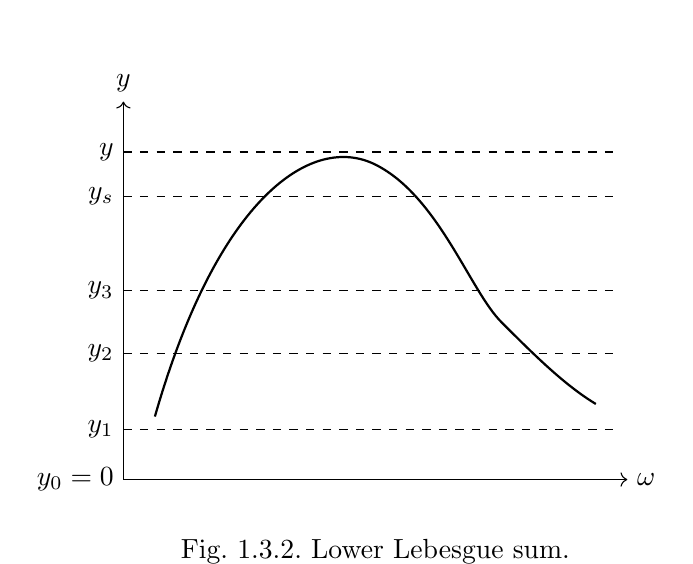
\begin{tikzpicture}[scale=0.8]
    % Axes
    \draw[->] (0,0) -- (8,0) node[right] {$\omega$};
    \draw[->] (0,0) -- (0,6) node[above] {$y$};

    % Curve (representing X(omega))
    \draw[thick] (0.5,1) .. controls (1.5,4.5) and (3,5.5) .. (4,5)
                 .. controls (5,4.5) and (5.5,3) .. (6,2.5)
                 .. controls (6.5,2) and (7,1.5) .. (7.5,1.2);

    % Horizontal dashed lines for y levels
    \draw[dashed] (0,0.8) -- (7.8,0.8);
    \draw[dashed] (0,2) -- (7.8,2);
    \draw[dashed] (0,3) -- (7.8,3);
    \draw[dashed] (0,4.5) -- (7.8,4.5);
    \draw[dashed] (0,5.2) -- (7.8,5.2);

    % Y-axis labels
    \node[left] at (0,0) {$y_0 = 0$};
    \node[left] at (0,0.8) {$y_1$};
    \node[left] at (0,2) {$y_2$};
    \node[left] at (0,3) {$y_3$};
    \node[left] at (0,4.5) {$y_s$};
    \node[left] at (0,5.2) {$y$};

    % Caption
    \node[below] at (4,-0.8) {Fig.\ 1.3.2.\ Lower Lebesgue sum.};
\end{tikzpicture}
\end{center}

\newpage
\section{Stochastic Processes: Preliminaries}
\label{sec:org04c7d97}

\subsection{Stochastic Processes}
\label{sec:org4879aa6}

\begin{definition}[stochastic process]
For a given probability space $(\Omega, \A, \P)$, a (real-valued) \textbf{stochastic process} $(X_t)_{t \in I}$ is a collection of $\A$-measurable random variables $X_t$ where $t \in I$ (known as the index set). It can also be written as $(X_{t,\omega})_{t \in I, \omega \in \Omega}$ to reflect that it is actually a function of two variables mapping from $I \times \Omega \to \R$.
\end{definition}

\begin{definition}[filtration, $\F$-adapted process, natural filtration]
\leavevmode
\begin{itemize}
    \item A \textbf{filtration} $\F = (\F_t)_{t \in [0,T]}$ is an increasing family of $\sigma$-algebras, that is, $\F_u \subseteq \F_t$ for any $0 \leq u \leq t \leq T$.
    \item A stochastic process $X = (X_t)_{t \in [0,T]}$ defined on $(\Omega, \F, \P)$ is \textbf{$\F$-adapted} if for any $t \in [0,T]$, the random variable $X_t$ is $\F_t$-measurable, i.e.\ for any $x \in \mathbb{Q}$, the event $\{X_t \leq x\} \in \F_t$ (Corollary~1.3.1).
    \item The \textbf{natural filtration} of $X$ (or the filtration generated by $X$) is defined as $\F^X = (\F^X_t)_{t \in [0,T]}$ where $\F^X_t = \sigma(X_u, u \leq t)$. Any stochastic process $X$ is, by definition, adapted to its natural filtration.
\end{itemize}
\end{definition}

\begin{remark}
We assume that $\A = \F_T$ and hereafter we shall write $(\Omega, \F, \P)$ instead of $(\Omega, \A, \F, \P)$.
\end{remark}

\begin{definition}[``equality'' of stochastic processes]
Two processes $X$ and $Y$ defined on a common probability space are said to be
\begin{itemize}
    \item (stronger) \textbf{indistinguishable} if the event $\{X_t = Y_t, \text{ for all } t \in [0,T]\}$ has probability 1, i.e.\ $\P\!\left(\bigcap_t \{X_t = Y_t\}\right) = 1$.
    \item (weaker) \textbf{modifications} of each other if for all $t \geq 0$, $\P(X_t = Y_t) = 1$.
\end{itemize}
\end{definition}

\begin{remark}
\leavevmode
\begin{enumerate}
    \item $X$ and $Y$ are indistinguishable $\Rightarrow$ $X$ and $Y$ are modifications of each other, but not the reverse.
    \item In discrete time these two concepts coincide.
\end{enumerate}
\end{remark}

\begin{proof}
We only need to show the converse. Since $X$ and $Y$ are modifications of each other, $\P(X_t = Y_t) = 1$ for all $t$ in some countable set $I$. Since countable unions of null sets are again null sets\footnote{Follows from countable additivity of probability measure (Definition~1.2.2).}, countable intersections of sets with full measure, have again full measure. Hence, $\P\!\left(\bigcap_{t \in I} \{X_t = Y_t\}\right) = 1$.
\end{proof}

\begin{enumerate}
    \setcounter{enumi}{2}
    \item If $X$ and $Y$ two c\`adl\`ag processes are modification of each other, then $X$ and $Y$ are indistinguishable.
\end{enumerate}

\begin{examples}[Counterexample of the converse]
We give an example where $X$ and $Y$ are modifications of each other, but not distinguishable. Consider the space $([0,1], \B([0,1]), \P)$, where $\P$ is the Lebesgue measure, i.e.\ $\P([a,b]) = b - a$. Let $(Y_t)_{t \in [0,1]}$ denote a constant process given by $Y_t = 0$ and $(X_t)_{t \in [0,1]}$ given by
\[
X_t(\omega) = \begin{cases} 1 & \text{if } t = \omega, \\ 0 & \text{if } t \neq \omega. \end{cases}
\]

For a fixed $\omega$, the trajectories $X_t(\omega)$ and $Y_t(\omega)$ differs only at the point $t = \omega$. To see that $X$ and $Y$ are modifications of each other, for every $t \in [0,1]$, we have
\[
\{\omega : X_t(\omega) = Y_t(\omega)\} = \{\omega : \omega \neq t\} = \Omega \setminus \{\omega : \omega = t\}
\]
This shows that $\P(X_t = Y_t) = 1 - \P(\{t\}) = 1$. Here the process $X$ is not a right continuous process (c\`adl\`ag), therefore one cannot conclude that $X$ and $Y$ are indistinguishable. In fact, we see that
\[
\{\omega : X_t(\omega) = Y_t(\omega), \text{ for all } t \in [0,1]\} = \bigcap_{t \in [0,1]} \{\omega : X_t(\omega) = Y_t(\omega)\} = \emptyset
\]
since the complement is given by
\[
\bigcup_{t \in [0,1]} \{\omega : X_t(\omega) \neq Y_t(\omega)\} = \bigcup_{t \in [0,1]} \{\omega : \omega = t\} = \Omega
\]
which means $(X_t)_{t \in [0,1]}$ and $(Y_t)_{t \in [0,1]}$ cannot be indistinguishable.
\end{examples}
\subsection{Martingales}
\label{sec:org67660db}

\begin{definition}[martingales, submartingales, supermartingales]
Consider a real-valued, $\F$-adapted process $M = (M_t)_{t \in [0,T]}$, defined on a filtered probability space $(\Omega, \F, \P)$. If
\begin{enumerate}[label=(\roman*)]
    \item $M$ is integrable, that is, $\E|M_t| < \infty$ for $t \in [0,T]$, and
    \item (martingale property) for any $0 \leq s \leq t \leq T$,
    \begin{itemize}
        \item $\E(M_t|\F_s) = M_s$, then $M$ is an $\F$-\textbf{martingale}. The expectation is a constant: $\E(M_t) = \E(M_0)$, for all $t \in [0,T]$.
        \item $\E(M_t|\F_s) \geq M_s$, then $M$ is an $\F$-\textbf{submartingale}. The expectation is increasing: $\E(M_t) \geq \E(M_0)$ for any $t \in [0,T]$.
        \item $\E(M_t|\F_s) \leq M_s$, then $M$ is an $\F$-\textbf{supermartingale}. The expectation is decreasing: $\E(M_t) \leq \E(M_0)$ for any $t \in [0,T]$.
    \end{itemize}
\end{enumerate}
\end{definition}

\begin{remark}
(equivalent conditions for discrete time martingales) For a discrete time process, it suffices to show
\begin{itemize}
    \item $\E(M_{n+1}|\F_n) = M_n$ for all $n = 0, 1, \ldots, N-1$, or
    \item $\E(M_N|\F_n) = M_n$ for all $n = 0, 1, \ldots, N$.
\end{itemize}
Other ways to prove a martingale in continuous case include:
\begin{itemize}
    \item Lemma~2.2.1: A sub- or supermartingale with constant expectation.
    \item $\E(M_T|\F_t) = M_t$ for all $t \in [0,T]$.
    \item Corollary~3.3.2: $M^2 - \langle M \rangle$ is an $\F$-martingale if $M$ is a continuous, square integrable $\F$-martingale.
    \item Theorem~4.1.1: $I(\gamma)$ for $\gamma \in L^2_\P(W)$ is an $\F$-martingale.
    \item Theorem~4.2.1: $I(\gamma)$ for $\gamma \in L_\P(W)$ is an $\F$-local martingale.
    \item It\^o's lemma (Theorem~4.3.1) proves a continuous semimartingale when $g$ is sufficiently smooth.
\end{itemize}
\end{remark}

\begin{lemma}
Assume that $M$ is either an $\F$-submartingale or an $\F$-supermartingale. Then $M$ is an $\F$-martingale if and only if the expected value of $M$ is constant, i.e.\ $\E[M_0] = \E[M_t]$ for all $t \in [0,T]$.
\end{lemma}

\begin{proof}
The only if part is straightforward. We prove only the converse.

Suppose $M$ is a submartingale with constant expectation. Let $0 \leq u \leq t \leq T$. Then $\E[M_t|\F_u] - M_u \geq 0$ and
\[
\E[\E[M_t|\F_u] - M_u] = \E[M_t] - \E[M_u] = 0
\]
by assumption. A non-negative random variable $X$ with $\E(X) = 0$ almost surely, as the Markov inequality implies $\P(X \geq 2^{-n}) \leq 2^n \E(X) = 0$.
This implies that $\E[M_t|\F_u] = M_u$ almost surely, i.e.\ $M$ is an $\F$-martingale.
\end{proof}

\begin{lemma}[convex transform of a martingale]
Let $M$ be an $\F$-martingale and let $h : \R \to \R$ be a convex function. If the process $X = h(M)$ is integrable, then it is an $\F$-submartingale.
\end{lemma}

\begin{examples}[Conditional Jensen's inequality (Theorem~1.5.2)]
Conditional Jensen's inequality can come handy when dealing with martingales. For example, if $S$ is a martingale, then the process $(S - K)^+$ is a submartingale, as $f : x \mapsto (x - K)^+$ is convex:
\[
\E[f(S_t)|\F_s] \geq f(\E[S_t|\F_s]) = f(S_s),
\]
for $0 \leq s \leq t \leq T$.
Similarly we can show that $(S^2)$ is also a submartingale.
\end{examples}

\begin{lemma}[conditional expectation process is a martingale]
Let $X$ be an $\F_T$-measurable and integrable random variable. Then the process defined by $M_t = \E(X|\F_t)$ for $t \in [0,T]$ is an $\F$-martingale.
\end{lemma}

\begin{proof}
This is an immediate result of the tower property.
\end{proof}
\subsection{Local Martingales}
\label{sec:org7a1e0e7}

\begin{definition}[local martingales]
A process $M$ is an $\F$-\textbf{local martingale} if there exists an increasing sequence $(\tau_n)_{n \in \mathbb{N}}$ of stopping times such that $\tau_n \to T$ a.s.\ ($T$ can be $\infty$), and for every $n$ the stopped process $M^{\tau_n}$ is a uniformly integrable martingale. Any sequence $(\tau_n)_{n \in \mathbb{N}}$ with these properties is called the \textbf{reducing sequence} for a local martingale $M$.
\end{definition}
\subsection{Doob Decomposition Theorem}
\label{sec:orgf9c4d7a}

\subsubsection{Discrete Time: Doob Decomposition}
\label{sec:orgc10e4a1}

\begin{theorem}[Doob decomposition theorem]
A discrete time submartingale $X = (X_n)_{n=0,1,\ldots,N}$ can be decomposed into
\[
X_n = M_n + A_n
\]
where $M$ is a martingale and $A$ is a predictable, increasing process with $A_0 = 0$. Similarly, a supermartingale can be decomposed into a martingale and a decreasing process. This decomposition is almost surely unique.
\end{theorem}

\begin{proof}
\textbf{Existence.} We prove the existence of Doob decomposition by construction. Define the processes $A$ and $M$ by setting, for every $n \in I = \{0, 1, \ldots, N\}$,
\[
A_n = \sum_{k=1}^{n} \left(\E[X_k|\F_{k-1}] - X_{k-1}\right)
\]
and
\[
M_n = X_0 + \sum_{k=1}^{n} \left(X_k - \E[X_k|\F_{k-1}]\right).
\]

It is easy to check that $X_n = M_n + A_n$ for all $n \in I$, by writing $X_n - X_0$ as a telescoping sum.

It is clear that $A$ is increasing since $\E[X_k|\F_{k-1}] - X_{k-1} \geq 0$. To check that $M$ is a martingale, we note that
\begin{align*}
\E[M_n|\F_{n-1}] &= \E[\hblue{M_{n-1} + X_n - \E[X_n|\F_{n-1}]} \mid \F_{n-1}] \\
&= M_{n-1} + \E[X_n|\F_{n-1}] - \E[X_n|\F_{n-1}] \\
&= M_{n-1}
\end{align*}
for all $n = 1, \ldots, N$.

\textbf{Uniqueness.} Let $X = M' + A'$ be an additional decomposition. Then the process $Y := M - M' = A' - A$ is a martingale, implying that
\[
\E[Y_n|\F_{n-1}] = Y_{n-1},
\]
and also predictable (as $A$ is predictable), implying that
\[
\E[Y_n|\F_{n-1}] = Y_n,
\]
for any $n = 1, \ldots, N$. Since $Y_0 = A'_0 - A_0 = 0$ by the convention about the starting point of the predictable processes, this implies iteratively that $Y_n = 0$ almost surely for all $n = 0, 1, \ldots, N$.
\end{proof}
\subsubsection{Continuous Time: Doob--Meyer Decomposition}
\label{sec:org29c8f00}

\begin{theorem}[Doob--Meyer decomposition theorem]
Let $X$ be a non-negative continuous submartingale\footnote{A more general version of the theorem applies to any c\`adl\`ag supermartingale of class D.}. Then there exists a continuous increasing process $A$ with $A_0 = 0$ such that the process $M = X - A$ is a continuous martingale. The processes $M$ and $A$ in the Doob--Meyer decomposition
\[
X = M + A
\]
are unique up to indistinguishability of stochastic processes (Definition~2.1.3).
\end{theorem}
\subsection{Stopping Times}
\label{sec:org2c4fb04}

\begin{definition}[stopping time]
An $\F$-\textbf{stopping time} $\tau$ is a random variable taking values in $[0, \infty]$ such that
\[
\{\tau \leq t\} \in \F_t
\]
for all $t \geq 0$.
\end{definition}

\begin{lemma}[stopped processes in discrete time, p.26]
\leavevmode
\begin{itemize}
    \item Let $X = (X_n)_{n=0,\ldots,N}$ be an $\F$-adapted process and $\tau$ be an $\F$-stopping time. Then the stopped process
    \[
    X^\tau := (X_{n \wedge \tau}) = X_n \indic_{n < \tau} + X_\tau \indic_{n \geq \tau}
    \]
    is also $\F$-adapted.
    \item Let $M = (M_n)_{n=0,\ldots,N}$ be an $\F$-martingale process and $\tau$ be an $\F$-stopping time. Then the stopped process
    \[
    M^\tau := (M_{n \wedge \tau}) = M_n \indic_{n < \tau} + M_\tau \indic_{n \geq \tau}
    \]
    is also an $\F$-martingale.
\end{itemize}
\end{lemma}

\begin{definition}
Given a stopping time $\tau$, the $\sigma$-algebra $\F_\tau$ defined by
\[
\F_\tau = \{A \in \F_T : \text{for all } t \in [0,T], \; A \cap \{\tau \leq t\} \in \F_t\}
\]
is called the \textbf{$\sigma$-algebra of events prior to $\tau$}.
\end{definition}

\begin{theorem}[Doob's optional sampling theorem]
Let $\sigma \leq \tau$ be two stopping times taking values in $\{0, 1, \ldots, N\}$. For any martingale, submartingale or supermartingale $X$, we have
\begin{enumerate}[label=(\roman*)]
    \item The random variables $X_\sigma$ and $X_\tau$ are integrable.
    \item $\E[X_\tau|\F_\sigma] = X_\sigma$ (if $X$ is a martingale), $\E[X_\tau|\F_\sigma] \geq X_\sigma$ (submartingale) and $\E[X_\tau|\F_\sigma] \leq X_\sigma$ (supermartingale) holds respectively.
\end{enumerate}
\end{theorem}

\begin{lemma}[a discrete time result]
Let $M = (M_n)_{n=0,1,\ldots,N}$ be an $\F$-adapted and integrable stochastic process. Then $M$ is an $\F$-martingale if and only if $\E(M_\tau) = \E(M_0)$ for any stopping time $\tau$ with values in $\{0, 1, \ldots, N\}$.
\end{lemma}

\begin{proof}
($\Rightarrow$) This is a direct result of Lemma~2.2.1.

($\Leftarrow$) By tower property, it suffices to check that $M_n = \E(M_N|\F_n)$ for every $n \in \{0, 1, \ldots, N\}$. By assumption, we have $\E(M_\tau) = \E(M_N)$ for any stopping time $\tau$ with values in $\{0, 1, \ldots, N\}$ (this is true since $\tau = N$ is also a stopping time). Let us fix $t$ and consider an event $A \in \F_t$. Define $\tau_A$ as
\[
\tau_A = \begin{cases} n, & \text{if } \omega \in A, \\ N, & \text{if } \omega \notin A, \end{cases}
\]
then $\tau_A$ is an $\F$-stopping time with values in $\{0, 1, \ldots, N\}$ and so $\E(M_{\tau_A}) = \E(M_N)$. This yields $\E(\indic_A M_n) = \E(\indic_A M_N)$. Since this equality holds for any event $A \in \F_t$, by definition we have $M_n = \E(M_N|\F_n)$, which in turn implies that $M$ is an $\F$-martingale.
\end{proof}

\newpage
\section{Brownian Motion}
\label{sec:org27dcb5e}

\subsection{Brownian Motion}
\label{sec:org0c6a77c}

\begin{definition}[standard Brownian motion]
A real-valued process $W = (W_t)_{t \in [0,T]}$, with $W_0 = 0$, defined on a filtered probability space $(\Omega, \F, \P)$, is called a standard $\F$-Brownian motion if:
\begin{enumerate}
    \item $W$ is $\F$-adapted.
    \item For any $0 \leq u \leq t \leq T$, $W_t - W_u$ is independent of $\F_u$.
    \item For any $0 \leq u \leq t \leq T$, $W_t - W_u \sim \N(0, t - u)$.
    \item $W$ is sample-paths continuous, i.e.\ almost all sample paths of $W$ are continuous.
\end{enumerate}
\end{definition}

\begin{definition}[Gaussian process]
A stochastic process $(X_t)_{t \geq 0}$ is said to be a Gaussian process, if for arbitrary times $0 < t_1 < t_2 < \cdots < t_n$, the vector $(X_{t_1}, \ldots, X_{t_n})$ follows a multivariate Gaussian distribution.
\end{definition}
\subsection{Properties of Brownian Motion}
\label{sec:org6d219c7}

\begin{theorem}[properties of Brownian motion]
Let $W$ be an $\F$-Brownian motion. Then
\begin{enumerate}
    \item \textbf{(martingale property)} $W$ is a continuous $\F$-martingale.
    \item \textbf{(Markov property)} For any bounded Borel measurable function $g : \R \to \R$ and $0 \leq u \leq t \leq T$,
    \[
    \E[g(W_t)|\F_u] = \E[g(W_t)|\sigma(W_u)] = \underbrace{h(W_u)}_{\text{Doob's measurability theorem}}
    \]
    \item $W$ is a Gaussian process.
    \item $\Cov(W_s, W_t) = \E[W_s W_t] = \min(s, t)$ for all $s, t \geq 0$ and in particular $\E[W_t^2] = t$.
\end{enumerate}
\end{theorem}

\begin{proof}
For (1), note that $W$ is an integrable, $\F$-adapted process with $\E(W_t|\F_u) = \E(W_t - W_u + W_u|\F_u) = W_u$ for any $0 \leq u \leq t \leq T$.

For (2),
\begin{align*}
\E[g(W_t)|\F_u] &= \E[g(W_t - W_u + W_u)|\F_u] \\
&= \E[g(W_t - W_u + x)|\F_u]\big|_{x=W_u} && \text{($W_u$ is $\F_u$-measurable)} \\
&= \E[g(W_t - W_u + x)]\big|_{x=W_u} && \text{(independent increments)}
\end{align*}
which is a function of $W_u$ and therefore $\sigma(W_u)$-measurable (Lemma~1.5.1). It follows that
\[
\E[\hblue{\E[g(W_t)|\F_u]}|\sigma(W_u)] = \hblue{\E[g(W_t)|\F_u]}
\]
\[
\Rightarrow \E[g(W_t)|\sigma(W_u)] = \E[g(W_t)|\F_u].
\]

For (3), note that
\[
\begin{pmatrix} W_{t_1} \\ W_{t_2} \\ \vdots \\ W_{t_n} \end{pmatrix}
=
\begin{pmatrix} 1 & 0 & \cdots & 0 \\ 1 & 1 & \cdots & 0 \\ \vdots & \vdots & \ddots & \vdots \\ 1 & 1 & \cdots & 1 \end{pmatrix}
\underbrace{\begin{pmatrix} W_{t_1} \\ W_{t_2} - W_{t_1} \\ \vdots \\ W_{t_n} - W_{t_{n-1}} \end{pmatrix}}_{=: y \sim \N}
\]
We can then conclude by using the fact that any linear transform of a Gaussian vector is again Gaussian. In particular, $(W_{t_1}, \ldots, W_{t_n}) \sim \N(0, A\Sigma A^T)$ where $\Sigma = \Var(y)$.

For (4),
\begin{align*}
\Cov(W_s, W_t) &= \E[W_s W_t] \\
&= \E[W_s(W_t - W_s)] + \E[W_s^2] \\
&= \E[W_s]\E[W_t - W_s] + \E[W_s^2] \\
&= s
\end{align*}
Similarly when $s \geq t$, $\Cov(W_s, W_t) = t$. Therefore $\E[W_t W_s] = \min(s, t)$.
\end{proof}

\begin{examples}[Exponential Brownian motion with drift]
Let $x, m \in \R$ and $\sigma > 0$ and we set $Y_t = x e^{mt + \sigma W_t}$. The process $Y$ is called an exponential Brownian motion with drift $m$ and variance $\sigma^2$. We first notice that the process $Y$ is adapted to the filtration $\F$. Next,
\[
\E[Y_t] = x e^{mt} \E(e^{\sigma W_t}) = x e^{mt} M_{W_t}(\sigma) = x e^{(m + \sigma^2/2)t}.
\]
We want to show that the process $Y$ is an $\F$-martingale if and only if $m = -\sigma^2/2$. Indeed, for $s \leq t$,
\begin{align*}
\E[x e^{mt + \sigma W_t} | \F_s] &= \E[x e^{ms + m(t-s) + \sigma W_s + \sigma(W_t - W_s)} | \F_s] \\
&= Y_s \E[e^{m(t-s) + \sigma(W_t - W_s)}] \\
&= Y_s e^{m(t-s) + \sigma^2(t-s)/2}
\end{align*}
and the claim follows.
\end{examples}
\subsection{Quadratic Variation}
\label{sec:org515348e}

\subsubsection{Total Variation}
\label{sec:org8172b54}

\begin{definition}[total variation, aka first-order variation]
Let $\pi_n = \{t_0 = 0, t_1, \ldots, t_{m_n} = T\}$ be a partition of $[0,T]$ with $n(\pi) = m_n$ subintervals. The maximum step size of the partition is denoted by
\[
|\pi_n| := \max_{1 \leq k \leq m_n} (t_k - t_{k-1}).
\]
For a given partition $\pi_n$, we define the corresponding measure of the oscillation of a function $f$ by
\[
V_n(f) = \sum_{k=1}^{m_n} |f(t_k) - f(t_{k-1})|.
\]
The total variation of $f$ is defined as
\[
V(f) := \lim_{|\pi_n| \to 0} V_n(f) = \lim_{|\pi_n| \to 0} \sum_{k=1}^{m_n} |f(t_k) - f(t_{k-1})|
\]
\end{definition}

\begin{lemma}
Any continuously differentiable function $f$ is a function of finite variation, i.e.\ $V(f) < \infty$.
\end{lemma}

\begin{proof}
\[
V_n(f) = \sum_{k=1}^{m_n} \left|\int_{t_{k-1}}^{t_k} f'(t) \, dt\right| \leq \sum_{k=1}^{m_n} \int_{t_{k-1}}^{t_k} |f'(t)| \, dt = \int_0^T |f'(t)| \, dt < \infty
\]
where we have used the fact that any continuous function on a closed and bounded interval is bounded. By taking the limit as $|\pi_n| \to 0$, we have proved that any continuously differentiable function $f$ on $[0,T]$ is a function of finite variation.
\end{proof}

\begin{theorem}[Jordan's decomposition and related results]
\leavevmode
\begin{itemize}
    \item Any bounded increasing function $f$ is a function of finite variation, i.e.\ $V(f) < \infty$.
    \item (Jordan's decomposition) If $f$ is a function of finite variation, i.e.\ $V(f) < \infty$, then $f = f_1 - f_2$ where $f_1, f_2$ are non-decreasing functions.
    \item The difference of two bounded increasing functions is a function of finite variation.
\end{itemize}
\end{theorem}

\begin{proof}
(Sketch) The first result comes from $V(f) = |f(T) - f(0)| < \infty$.

The second result can be proved by construction (omitted).

The third result follows from (1) as well as the fact that the difference of two functions of finite variation also has finite variation (a direct result of triangle inequality).
\end{proof}
\subsubsection{Quadratic Variation}
\label{sec:org7f962d5}

\begin{definition}[quadratic variation]
For a given partition $\pi_n = \{t_0 = 0, t_1, \ldots, t_{m_n} = T\}$ of $[0,T]$, the quadratic variation of $f$ is defined as
\[
\langle f \rangle = V^{(2)}(f) := \lim_{|\pi_n| \to 0} V_n^{(2)}(f) = \lim_{|\pi_n| \to 0} \sum_{k=1}^{m_n} |f(t_k) - f(t_{k-1})|^2
\]
\end{definition}

\begin{lemma}
Any continuously differentiable function $f$ has zero quadratic variation, i.e.\ $V^{(2)}(f) = 0$.
\end{lemma}

\begin{proof}
\[
V_n^{(2)}(f) = \sum_{k=1}^{m_n} |f(t_k) - f(t_{k-1})|^2 = \sum_{k=1}^{m_n} \left(\int_{t_{k-1}}^{t_k} f'(t) \, dt\right)^2
\]
\[
\leq \sum_{k=1}^{m_n} (t_k - t_{k-1}) \int_{t_{k-1}}^{t_k} |f'(t)|^2 \, dt \qquad \text{(by Cauchy--Schwarz, see Theorem~A.0.1)}
\]
\[
\leq |\pi_n| \int_0^T |f'(t)|^2 \, dt < \infty
\]
Taking the limit as $|\pi_n| \to 0$, we have $V^{(2)}(f) = \lim_{|\pi_n| \to 0} V_n^{(2)}(f) = 0$, completing the proof. Alternatively, this can also be shown by combining the results of Lemma~3.3.1 and~3.3.3.
\end{proof}

\begin{lemma}[finite variation $\Rightarrow$ zero quadratic variation]
Let $f$ be a continuous function of finite variation on $[0,T]$. Then the quadratic variation of $f$ is equal to zero.
\end{lemma}

\begin{proof}
Observe that for any partition $\pi_n = \{t_0 = 0, t_1, \ldots, t_{m_n} = T\}$ of $[0,T]$ we have
\begin{align*}
V_n^{(2)}(f) &= \sum_{k=1}^{m_n} |f(t_k) - f(t_{k-1})|^2 \\
&\leq \max_{1 \leq m \leq m_n} |f(t_m) - f(t_{m-1})| \sum_{k=1}^{m_n} |f(t_k) - f(t_{k-1})| \\
&= \max_{1 \leq m \leq m_n} |f(t_m) - f(t_{m-1})| \cdot V_n(f).
\end{align*}
By using the fact that any continuous function is uniformly continuous on a closed bounded interval, taking the limit as $|\pi_n| \to 0$ completes the proof.
\end{proof}

\begin{corollary}
(from Lemma~3.3.3) If the quadratic variation of a continuous stochastic process is a.s.\ strictly positive, then the total variation of the process is almost surely infinity. In particular, sample paths of a Brownian motion are a.s.\ functions of infinite variation on any interval.
\end{corollary}

\begin{theorem}
Let $W$ be a standard Brownian motion. $W$ is a process of finite quadratic variation. In particular, $\langle W \rangle_t = t$ (a.s.) for all $t \geq 0$.
\end{theorem}

\begin{proof}
Let $t \geq 0$ and $\pi_n = \{t_0 = 0, t_1, \ldots, t_{n(\pi)} = t\}$ be a partition of $[0,t]$. We want to show that
\[
\lim_{n(\pi) \to \infty} \sum_{k=1}^{n(\pi)} (W_{t_k} - W_{t_{k-1}})^2 =: V_n^{(2)}(W) = t
\]
where the convergence is in $L^2(\Omega, \F_T, \P)$, that is,
\[
\lim_{n(\pi) \to \infty} \E\left[\left(\sum_{k=1}^{n(\pi)} (W_{t_k} - W_{t_{k-1}})^2 - t\right)^2\right] = 0.
\]
For brevity of notation, write $\Delta t_k = t_k - t_{k-1}$, $\Delta W_k = W_{t_k} - W_{t_{k-1}}$ and $\theta_k = (\Delta W_k)^2 - \Delta t_k$. Our goal is to prove that $I_n = \E[(\sum \theta_k)^2] \to 0$ as $n(\pi) \to \infty$. To show this,
\[
I_n = \E\left[\left(\sum_{k=1}^{n(\pi)} \theta_k\right)^2\right] = \E\left[\sum_{i,j} \theta_i \theta_j\right] = \sum_{i=1}^{n(\pi)} \E(\theta_i^2) + 2\sum_{i \neq j} \E(\theta_i \theta_j)
\]
We can show that the second term is $0$ by using independent increments and $\E[(\Delta W_k)^2] = \Delta t_k$. Then
\begin{align*}
I_n &= \sum_{k=1}^{n(\pi)} \left(\E[(\Delta W_k)^4] - 2\Delta t_k \E[(\Delta W_k)^2] + (\Delta t_k)^2\right) \\
&= 2\sum_{k=1}^{n(\pi)} (\Delta t_k)^2 \leq 2|\pi_n| \sum_{k=1}^{n(\pi)} \Delta t_k = 2t|\pi_n|
\end{align*}
where in the second equality we used the fact the 4th central moment of a $X \sim \N(\mu, \sigma^2)$ r.v.\ is $\E((X - \mu)^4) = 3\sigma^4$.

It is now clear that the quantity $I_n$ tends to zero as $n$ tends to infinity, since $|\pi_n|$ tends to zero.
\end{proof}

\begin{lemma}
The process $M = W^2 - \langle W \rangle$ is a continuous $\F$-martingale.
\end{lemma}

\begin{proof}
The process $M$ is $\F$-adapted and integrable since $W^2$ is $\F$-adapted and integrable, while the quadratic variation $\langle W \rangle_t = t$ is clearly $\F$-adapted and integrable.

For $0 \leq u \leq t \leq T$, from the equality $\E(W_t W_u|\F_u) = W_u \E(W_t|\F_u) = W_u^2$, we deduce that
\begin{align*}
\E(M_t|\F_u) &= \E(W_t^2 - t|\F_u) \\
&= \E(W_t^2 - W_u^2 + W_u^2 - t|\F_u) \\
&= \E(W_t^2 - W_u^2|\F_u) + W_u^2 - t \\
&= \E((W_t - W_u)^2|\F_u) + W_u^2 - t \\
&= W_u^2 - u = M_u.
\end{align*}
\end{proof}

\begin{theorem}[alternative definition of quadratic variation for martingales]
Let $M$ be a continuous, square integrable $\F$-martingale, i.e.\ $\E(M_t^2) < \infty$ for all $t \geq 0$. Then the quadratic variation $\langle M \rangle$ is the unique continuous, increasing and $\F$-adapted process with $\langle M \rangle_0 = 0$ such that $M^2 - \langle M \rangle$ give us an $\F$-martingale.
\end{theorem}

\begin{remark}
The existence of $\langle M \rangle$ in the theorem above follows from the Doob--Meyer decomposition (Theorem~2.4.2).
\end{remark}

We now obtain a generalisation of Lemma~3.3.4:

\begin{corollary}
(from Theorem~3.3.3) If $M$ is a continuous, square integrable $\F$-martingale, then
\[
M^2 - \langle M \rangle
\]
is also an $\F$-martingale. In particular, if $M_0 = 0$, then $\E[M_t^2 - \langle M \rangle_t] = M_0^2 - \langle M \rangle_0 = 0$ and therefore
\[
\Var(M_t) = \E(M_t^2) = \E(\langle M \rangle_t).
\]
\end{corollary}
\subsection{Reflection Principle}
\label{sec:org4558e86}

Let $b > 0$ and $B$ a standard Brownian motion. Define the hitting time
\[
T_b = \inf\{s : B_s = b\}.
\]

\begin{theorem}
The following results hold (pp.41--44):
\begin{itemize}
    \item \textbf{(reflection principle)} $\P(T_b < t) = 2\P(B_t > b)$. More precisely, $T_b$ follows a L\'{e}vy distribution with parameters $(0, b^2)$ (or equivalently, an inverse Gamma distribution with shape $1/2$ and scale $b^2$).
    \item We can therefore show that $\P(T_b < \infty) = 1$ but $\E(T_b) = \infty$.
    \item The moment generating function of $T_b$ is $e^{-\sqrt{2\lambda}\, b}$ for $b, \lambda > 0$.
    \item For any $t \geq 0$, the running supremum $B_t^* = \sup_{s \leq t} B_s$ and $|B_t|$ have the same distribution.
    \item The joint distribution of $B_t^* = \sup_{s \leq t} B_s$ and $B_t$ is given by
    \[
    \P(B_t \leq x, B_t^* > y) = \P(B_t > 2y - x) = \P(B_t < x - 2y)
    \]
    for every $t \geq 0$, $y \geq 0$ and $x \leq y$.
    \item The joint density of $B_t^* = \sup_{s \leq t} B_s$ and $B_t$ is given by
    \[
    \frac{2(2y - x)}{t} \cdot \frac{1}{\sqrt{2\pi t}} \exp\!\left(-\frac{(2y - x)^2}{2t}\right)
    \]
    for $x \leq y$, $y \geq 0$.
    \item The drawdown $B_t^* - B_t$ has the same distribution as $|B_t|$.
\end{itemize}
\end{theorem}

\newpage
\section{Ito's Integral}\footnote{I will skip the definition of Ito's integral for elementary processes, which is required to formally define Ito's integral for more general processes as discussed here.}
\subsection{Ito's Integral for Processes from \(L^2_\P(W)\)}
\label{sec:orgdaadcaf}

\begin{definition}
$L^2_\P(W)$ denotes the class of all $\F$-progressively measurable processes $\gamma$ defined on $(\Omega, \F, \P)$ s.t.
\[
\|\gamma\|^2_W := \E\left[\int_0^T |\gamma_u|^2 \, du\right] < \infty.
\]
\end{definition}

\begin{definition}[Ito's integral for general integrands]
For any process $\gamma \in L^2_\P(W)$, the random variable $I_T(\gamma)$ is called Ito's integral of $\gamma$ with respect to $W$ over $[0,T]$. We write (notation only, not a formal definition):
\[
I_T(\gamma) = \int_0^T \gamma_u \cdot dW_u
\]
\[
I_t(\gamma) = I_T(\gamma \indic_{[0,t]}) = \int_0^t \gamma_u \cdot dW_u
\]
\end{definition}

\begin{theorem}[properties of Ito's integrals]
Let $\gamma \in L^2_\P(W)$, i.e.\ $\E\left[\int_0^T |\gamma_u|^2 \, du\right] < \infty$. Then:
\begin{enumerate}[label=(\roman*)]
    \item \hred{\textbf{(martingale)} $I(\gamma)$ is a continuous, square integrable $\F$-martingale.}

    \item \textbf{(linearity)} For constants $a$ and $b$, $I_t(a\gamma + b\eta) = aI_t(\gamma) + bI_t(\eta)$.

    \item \textbf{(Ito isometry)} $\E[I_t^2(\gamma)] = \E\left[\int_0^t \gamma_u^2 \, du\right]$.

    \item \textbf{(quadratic variation)} The quadratic variation accumulated up to time $t$ by the Ito's integral is
    \[
    \langle I(\gamma) \rangle_t = \int_0^t \gamma_u^2 \, du.
    \]
    Furthermore, Theorem~3.3.3 says that $I^2(\gamma) - \langle I(\gamma) \rangle$ is an $\F$-martingale. Corollary~3.3.2 implies that
    \[
    \Var(I_t(\gamma)) = \E[I_t^2(\gamma)] = \E[\langle I(\gamma) \rangle_t].
    \]

    \item \textbf{(local property)} For any $\F$-stopping time $\tau$, $I(\gamma \indic_{[0,\tau]}) = I_\tau(\gamma)$.
\end{enumerate}
\end{theorem}

\begin{proof}
For (iii), we prove the case for an elementary process $\gamma \in \mathcal{R}$. Since the expected value of the cross terms are zero, i.e.\ $\E[(W_{t_{j+1}} - W_{t_j})(W_{t_{k+1}} - W_{t_k})] = 0$ for $j \neq k$, we obtain
\begin{align*}
\E\left[\left(\sum_{j=0}^{m-1} \gamma_j (W_{t_{j+1}} - W_{t_j})\right)^2\right]
&= \E\left[\sum_{j=0}^{m-1} \gamma_j^2 (W_{t_{j+1}} - W_{t_j})^2\right] \\
&= \E\left[\sum_{i=0}^{m-1} \gamma_j^2 \E\left[(W_{t_{j+1}} - W_{t_j})^2 \mid \F_{t_j}\right]\right] \\
&= \E\left[\sum_{i=0}^{m-1} \gamma_j^2 (t_{j+1} - t_j)\right] \\
&= \|\gamma\|^2_W
\end{align*}
This means that $\hat{I}_T : (\mathcal{K}, \|\cdot\|_W) \to L^2(\Omega, \F_T, \P)$ is an isometry, i.e.\ a distance preserving transformation. This can be extended to the isometry $I_T : (L^2_\P(W), \|\cdot\|_W) \to L^2(\Omega, \F_T, \P)$.\footnote{The extension is done using the fact that the class of simple process $\mathcal{K}$ is a dense subset in the Banach space $L^2_\P(W)$ and the space $L^2(\Omega, \F_T, \P)$ is also complete (since it a Banach space or more specifically a Hilbert space).}

For (iv), again we consider an elementary process $\gamma$ and we can then do a similar proof to that of Theorem~3.3.2. We first compute the quadratic variation accumulated by the Ito integral on one of the subintervals $[t_j, t_{j+1}]$ on which $\gamma_u = \gamma_j$ is constant. For this, we choose partition points
\[
t_j = s_0 < s_1 < \cdots < s_m = t_{j+1}
\]
and consider
\[
\sum_{i=0}^{m-1} (I_{s_{i+1}}(\gamma) - I_{s_i}(\gamma))^2 = \sum_{i=0}^{m-1} (\gamma_j (W_{s_{i+1}} - W_{s_i}))^2 = \gamma_j^2 \sum_{i=0}^{m-1} (W_{s_{i+1}} - W_{s_i})^2
\]
As $m \to \infty$ and the step size $\max_{0 \leq i \leq m-1} (s_{i+1} - s_i)$ approaches zero, the term $\sum_{i=0}^{m-1} (W_{s_{i+1}} - W_{s_i})^2$ converges to the quadratic variation accumulated by Brownian motion between times $t_j$ and $t_{j+1}$, which is $t_{j+1} - t_j$. Therefore, the limit of the above is
\[
\gamma_j^2 (t_{j+1} - t_j) = \int_{t_j}^{t_{j+1}} \gamma_u^2 \, du.
\]
Adding up all these pieces for each of the subintervals $[t_j, t_{j+1}]$ completes the proof.
\end{proof}

\begin{examples}[Ito's integral for a deterministic integrand]
For a deterministic function $f$, we have
\[
X_t = \int_0^t f(s) \, dW_s \sim \N\left(0, \int_0^t f^2(s) \, ds\right).
\]
The computation of $\E(X_t)$ and $\Var(X_t)$ follows directly from Theorem~4.1.1. Normality follows from the fact that $X_t$ is (the limit of) the sum of independent normal r.v.s:
\[
\int_0^t f(s) \, dW_s = \lim_{m \to \infty} \sum_{j=0}^{m-1} f(t_j)(W_{t_{j+1}} - W_{t_j}).
\]
\end{examples}

\begin{examples}[Ito's integral]
We can show that $\int_0^t 2W_s \, dW_s$ is a martingale, by noting that
\[
\E\left[\int_0^T |2W_u|^2 \, du\right] = \int_0^T \E[4W_t^2] \, dt = \int_0^T 4t \, dt = 2T^2 < \infty
\]
where the first equality uses Fubini's Theorem.
\end{examples}
\subsection{Ito's Integral for Processes from \(L_\P(W)\)}
\label{sec:orgedb445e}

\begin{definition}
$L_\P(W)$ denotes the class of all $\F$-progressively measurable processes $\gamma$ on $(\Omega, \F, \P)$ s.t.
\[
\P\left(\int_0^T |\gamma_u|^2 \, du < \infty\right) = 1.
\]
\end{definition}

By applying the optional stopping technique (aka localisation), we can extend the definition of Ito's integral to the more general class $L_\P(W)$. Details are omitted, the important conclusion is that:

\begin{theorem}
\hred{If $\gamma \in L_\P(W)$, i.e.\ $\P\left(\int_0^T |\gamma_u|^2 \, du < \infty\right) = 1$, then $I(\gamma)$ is a continuous $\F$-local martingale.}
\end{theorem}
\subsection{Ito's Lemma in 1D}
\label{sec:org67b90a8}

Ito processes are a special class of continuous semimartingales.

\begin{definition}[Ito process]
An $\F$-adapted continuous process $X$ is called an Ito process if it admits a representation
\[
X_t = X_0 + \int_0^t \alpha_u \, du + \int_0^t \beta_u \cdot dW_u, \quad \text{for all } t \in [0,T]
\]
for some $\F$-adapted processes $\alpha$ and $\beta$ that are defined on $(\Omega, \F, \P)$ and satisfy suitable integrability conditions. It is customary to write the integral formula above using differential notation as
\[
dX_t = \alpha_t \, dt + \beta_t \cdot dW_t.
\]
\end{definition}

\begin{lemma}[quadratic variation of Ito processes]
Consider an Ito process denoted by $dX_t = \alpha_t \, dt + \beta_t \cdot dW_t$.
\begin{enumerate}[label=(\roman*)]
    \item The quadratic variation of the Ito process is $\langle X \rangle_t = \int_0^t \beta_u^2 \, du$.

    \item The quadratic covariation (aka cross-variation) of two Ito processes $X_t = \int_0^t \alpha_u \, dW_u$ and $Y_t = \int_0^t \beta_u \, dW_u$ is
    \[
    \langle X, Y \rangle_t = \int_0^t \alpha_u \beta_u \, du.
    \]

    \item \textbf{(polarisation formula)} A more general version of (ii) gives the quadratic covariation of two continuous semimartingales. If $X^i = X_0^i + M^i + A^i$ and $X^j = X_0^j + M^j + A^j$ are in $\Sc(\P)$, then
    \[
    \langle X^i, X^j \rangle = \langle M^i, M^j \rangle = \frac{1}{2}\left(\langle M^i + M^j \rangle - \langle M^i \rangle - \langle M^j \rangle\right) = \frac{1}{4}\left(\langle M^i + M^j \rangle - \langle M^i - M^j \rangle\right).
    \]
\end{enumerate}
\end{lemma}

\begin{proof}
(i) First note that the process $A_t = \int_0^t \alpha_u \, du$ is always a process of finite variation (thus zero quadratic variation). This is clear when $\alpha \geq 0$ and $A_t$ is increasing, since the total variation on $[0,T]$ is just $A_T$ (Theorem~3.3.1). If $\alpha$ is not positive, we can write $\alpha = \alpha^+ - \alpha^-$ and $A_t = A_t^+ - A_t^-$ where $\alpha^+ = \max(\alpha, 0)$, $\alpha^- = \max(-\alpha, 0)$ and
\[
A_t^{\pm} = \int_0^t \alpha_s^{\pm} \, ds
\]
and it is not difficult to see that the total variation of $A$ is bounded by $A_T^+ + A_T^-$.
The quadratic variation of the process $B_t = \int_0^t \beta_u \cdot dW_u$ is given in Theorem~4.1.1, thus the result.

(ii) We can use the polarisation formula:
\begin{align*}
\langle X, Y \rangle_t &= \frac{1}{2} \left(\langle X + Y \rangle_t - \langle X \rangle_t - \langle Y \rangle_t\right) \\
&= \frac{1}{2} \left(\left\langle \int (\alpha_u + \beta_u) \, dW_u, \int (\alpha_u + \beta_u) \, dW_u \right\rangle_t - \left\langle \int \alpha_u \, dW_u \right\rangle_t - \left\langle \int \beta_u \, dW_u \right\rangle_t\right) \\
&= \frac{1}{2} \left(\int_0^t (\alpha_u + \beta_u)^2 \, ds - \int_0^t \alpha_u^2 \, ds - \int_0^t \beta_u^2 \, ds\right) \\
&= \int_0^t \alpha_u \beta_u \, ds,
\end{align*}
which concludes the proof.
\end{proof}

\begin{theorem}[Ito's Lemma, 1D]
Suppose that $g : [0,T] \times \R \to \R$ is a function of class $C^{2,1}([0,T] \times \R, \R)$, i.e.\ $g$ is twice continuously differentiable. Then for any Ito process $X$, the process $Y_t = g(t, X_t)$, $t \in [0,T]$, is an Ito process (and therefore also a continuous semimartingale). Moreover, its canonical decomposition is given by the Ito formula
\[
dg(t, X_t) = g_t(t, X_t) \, dt + g_x(t, X_t) \, dX_t + \frac{1}{2} g_{xx}(t, X_t) \, d\langle X \rangle_t.
\]
or equivalently,
\[
g(t, X_t) = g(0, X_0) + \int_0^t g_t(s, X_s) \, ds + \int_0^t g_x(s, X_s) \, dX_s + \frac{1}{2} \int_0^t g_{xx}(s, X_s) \, d\langle X \rangle_s.
\]
If $dX_t = \alpha_t \, dt + \beta_t \, dW_t$, then
\[
dg(t, X_t) = g_t(t, X_t) \, dt + g_x(t, X_t) \alpha_t \, dt + g_x(t, X_t) \beta_t \, dW_t + \frac{1}{2} g_{xx}(t, X_t) \beta_t^2 \, dt.
\]
\end{theorem}

\begin{examples}[Ito's lemma, 1D]
We can use Ito formula to determine whether a process is a martingale (no drift), submartingale (drift $> 0$) or supermartingale (drift $< 0$).

\begin{enumerate}
    \item $f(W_t) = (W_t)^2$. Then we have for all $t \in [0,T]$,
    \[
    df(W_t) = 2W_t \, dW_t + \frac{1}{2} \cdot 2 \, dt \implies W_t^2 = W_0^2 + \int_0^t 2W_s \, dW_s + \int_0^t ds = \int_0^t 2W_s \, dW_s + t.
    \]
    This also gives the Doob--Meyer decomposition (Theorem~2.4.2) of the positive submartingale $W^2$. Also recall that $W_t^2 - t = \int_0^t 2W_s \, dW_s$ is a martingale (e.g.\ Theorem~3.3.3, or Example~4.1.2).

    \item $Y_t = g(t, W_t) = e^{\mu t + W_t}$. Let $g(t, x) = e^{\mu t + x}$ and then $g_t = \mu Y_t$, $g_x = Y_t$, $g_{xx} = Y_t$ and so
    \begin{align*}
    dY_t &= \mu Y_t \, dt + Y_t \, dW_t + \frac{1}{2} \cdot Y_t \, d\langle W \rangle_t = \left(\mu + \frac{1}{2}\right) Y_t \, dt + Y_t \, dW_t \\
    &\implies Y_t = Y_0 + \int_0^t \underbrace{\left(\mu + \frac{1}{2}\right) Y_u \, du}_{\text{increasing}} + \int_0^t \underbrace{Y_u \, dW_u}_{\text{a martingale, as } Y \in L^2_\P(W)}.
    \end{align*}
    Therefore, we conclude that $Y$ is a submartingale.

    \item (integration by parts, Corollary~4.4.1) $Z_t = \sin(W_t) \cos(W_t)$. Then
    \[
    dZ_t = \sin W_t \, d(\cos W_t) + \cos W_t \, d(\sin W_t) + d\langle \sin W, \cos W \rangle_t.
    \]
    By Ito's lemma,
    \begin{align*}
    d(\cos W_t) &= -\sin W_t \, dW_t - \frac{1}{2} \cos W_t \, dt, \\
    d(\sin W_t) &= \cos W_t \, dW_t - \frac{1}{2} \sin W_t \, dt.
    \end{align*}
    Also $d\langle \sin W, \cos W \rangle_t = -\sin W_t \cos W_t \, dt$, so
    \[
    dZ_t = -\sin^2(W_t) \, dW_t + \cos^2(W_t) \, dW_t - 2 \sin W_t \cos W_t \, dt
    \]
    The sign of the drift term is not always positive or negative, and therefore $Z$ is none of a martingale, submartingale or supermartingale.
\end{enumerate}
\end{examples}
\subsection{Ito's Lemma in Multidimensional Space}
\label{sec:org06abedf}

\begin{definition}[Ito's integral, multidimensional]
Let $\gamma \in L_W(\P)$, that is, $\gamma$ is an $\R^d$-valued $\F$-progressively measurable process satisfying
\[
\P\left(\int_0^T |\gamma_u|^2 \, du < \infty\right) = 1,
\]
where $|\cdot|$ stands for the Euclidean norm in $\R^d$. Then the Ito stochastic integral of $\gamma$ w.r.t.\ $W$ is well defined and for any $t \in [0,T]$,
\[
I_t(\gamma) = \int_0^t \gamma_u \cdot dW_u = \sum_{i=1}^{d} \int_0^t \gamma_u^i \, dW_u^i.
\]
\end{definition}

\begin{definition}[Ito process, multidimensional]
$X = (X^1, \ldots, X^k)$ is a $k$-dimensional Ito process if
\[
X_t^i = X_0^i + \int_0^t \alpha_u^i \, du + \int_0^t \beta_u^i \cdot dW_u
\]
where $\alpha^i$ are real-valued processes and $\beta^i = (\beta^{i1}, \ldots, \beta^{id})$ are $\R^d$-valued processes for $i = 1, \ldots, k$. It is implicitly assumed in the above that the processes $\alpha^i$, $\beta^i$, $i = 1, \ldots, k$ are integrable in a suitable sense.
\end{definition}

\begin{lemma}[quadratic variation of $k$-dimensional Ito processes]
For $X = (X^1, \ldots, X^k)$ defined in Definition~4.4.2, for any $t \in [0,T]$,
\[
\langle X^i, X^j \rangle_t = \int_0^t \beta_u^i \cdot \beta_u^j \, du = \int_0^t \sum_{l=1}^{d} \beta_u^{il} \beta_u^{jl} \, du.
\]
\end{lemma}

\begin{theorem}[Ito's Lemma, multidimensional]
Suppose that $g$ is a function of class $C^2(\R^k, \R)$, i.e.\ $g$ is twice continuously differentiable, and that $X$ a $k$-dimensional Ito process. Then
\begin{align*}
dg(X_t) &= \sum_{i=1}^{k} g_{x_i}(X_t) \, dX_t^i + \frac{1}{2} \sum_{i,j=1}^{k} g_{x_i x_j}(X_t) \beta_t^i \cdot \beta_t^j \, dt \\
&= \sum_{i=1}^{k} g_{x_i}(X_t) \alpha_t^i \, dt + \sum_{i=1}^{k} g_{x_i}(X_t) \beta_t^i \cdot dW_t + \frac{1}{2} \sum_{i,j=1}^{k} g_{x_i x_j}(X_t) \beta_t^i \cdot \beta_t^j \, dt.
\end{align*}
\end{theorem}

\begin{corollary}[integration by parts formula]
Given two continuous semimartingales $X$ and $Y$, then
\[
X_t Y_t = X_0 Y_0 + \int_0^t X_u \, dY_u + \int_0^t Y_u \, dX_u + \langle X, Y \rangle_t
\]
or equivalently,
\[
dX_t Y_t = X_t \, dY_t + Y_t \, dX_t + d\langle X, Y \rangle_t.
\]
If at least one of $X$ or $Y$ is a process of finite variation, then
\[
dX_t Y_t = X_t \, dY_t + Y_t \, dX_t.
\]
\end{corollary}

\begin{examples}[Ito's lemma, multidimensional]
Let
\[
R_t(d) := \sqrt{(W_t^1)^2 + (W_t^2)^2 + \cdots + (W_t^d)^2}
\]
where $W = (W^1, W^2, \ldots, W^d)$ is a standard $d$-dimensional Brownian motion for $d \geq 3$. The process $R$ is called a Bessel process. We want to show that $1/R_t(3)$ for $1 \leq t \leq T$ is a local martingale but not a martingale.

\begin{enumerate}
    \item To show it is a local martingale, we apply Ito's lemma to compute the dynamics of $1/R_t(3)$ (and show that there is no drift term). Let
    \[
    Y_t = R_t^2(3) = (W_t^1)^2 + (W_t^2)^2 + (W_t^3)^2 \implies dY_t = \sum_{i=1}^{3} 2W_t^i \, dW_t^i + 3 \, dt.
    \]
    But $1/R_t(3) = 1/\sqrt{Y_t} = g(Y_t)$ where $g(x) = 1/\sqrt{x}$. Strictly speaking, one cannot apply directly Ito's formula as $g$ is not differentiable at zero. But for $d \geq 3$, the $d$-dimensional Brownian motion never return to the origin after time $0$. So (heuristically) one can apply Ito formula again to obtain that
    \begin{align*}
    d(1/R_t(3)) &= -\frac{1}{2} \frac{1}{Y_t^{3/2}} \, dY_t + \frac{1}{2} \cdot \frac{3}{4} \cdot \frac{1}{Y_t^{5/2}} \, d\langle Y \rangle_t \\
    &= -\frac{1}{2} \frac{1}{Y_t^{3/2}} \left(\sum_{i=1}^{3} 2W_t^i \, dW_t^i + 3 \, dt\right) + \frac{1}{2} \cdot \frac{3}{4} \cdot \frac{1}{Y_t^{5/2}} (4Y_t \, dt) \\
    &= \frac{1}{R_t^3} \sum_{i=1}^{3} W_t^i \, dW_t^i = \frac{1}{R_t^3} W_t \cdot dW_t
    \end{align*}
    as $d\langle Y \rangle_t = \sum_{i=1}^{3} (2W_t^i)^2 \, dt = 4R_t^2 \, dt$. This is not a true martingale as $\|1/R_t^3 \cdot W_t\|^2_W = \infty$.

    \item We can also show that
    \[
    \E[1/R_t(d)] = \frac{1}{\sqrt{t}} \E\left[\frac{1}{\sqrt{X}}\right] = \sqrt{\frac{2}{\pi t}}
    \]
    where $X \sim \chi^2_3$. As the expectation is decreasing in $t$, $1/R_t(3)$ is indeed a supermartingale (see also Theorem~5.1.1).
\end{enumerate}
\end{examples}

\newpage
\section{Semimartingales}
\label{sec:orge4557d2}

\begin{center}
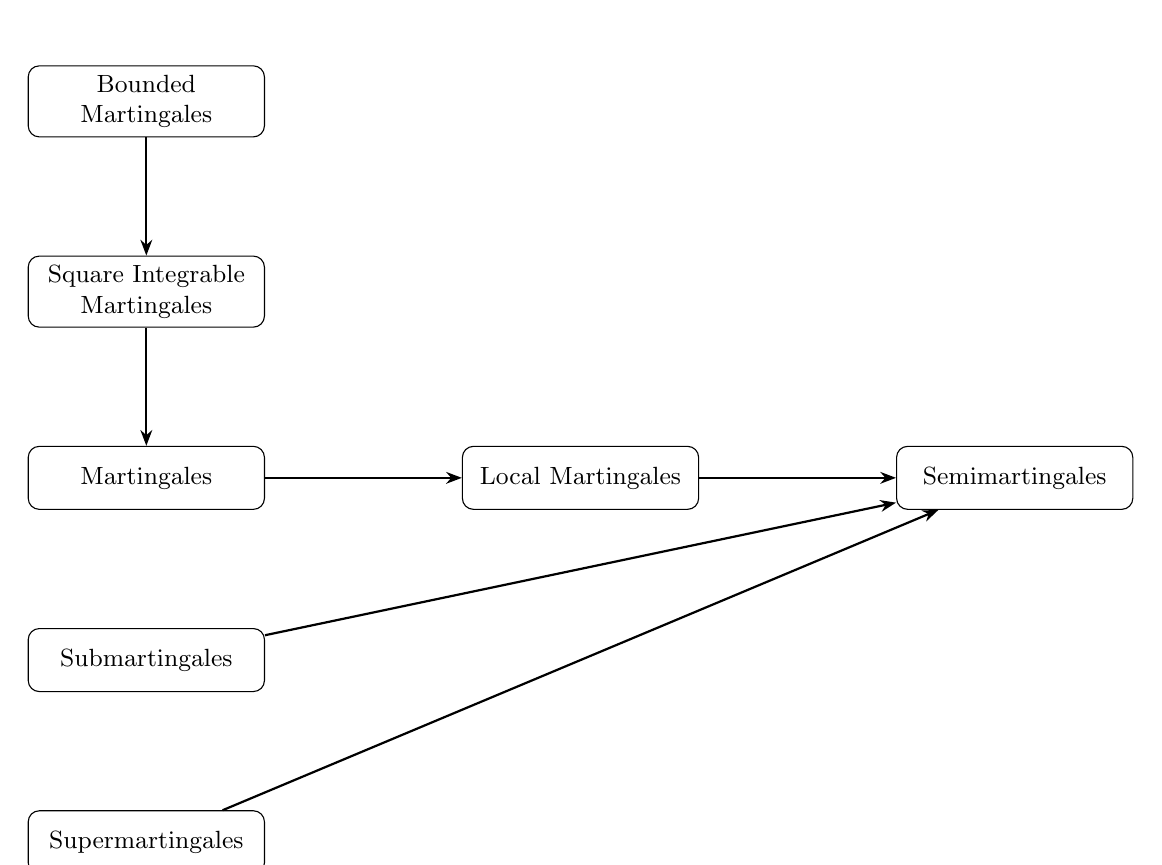
\begin{tikzpicture}[
    node distance=1.5cm and 2.5cm,
    box/.style={rectangle, draw, rounded corners, minimum width=3cm, minimum height=0.8cm, align=center, font=\small},
    arrow/.style={-{Stealth[length=2mm]}, thick}
]
    % Nodes
    \node[box] (mg) {Martingales};
    \node[box, right=of mg] (lmg) {Local Martingales};
    \node[box, right=of lmg] (smg) {Semimartingales};
    \node[box, above=of mg] (sqmg) {Square Integrable\\Martingales};
    \node[box, above=of sqmg] (bddmg) {Bounded\\Martingales};
    \node[box, below=of mg] (submg) {Submartingales};
    \node[box, below=of submg] (supmg) {Supermartingales};

    % Arrows (A -> B means A is a subclass of B)
    \draw[arrow] (bddmg) -- (sqmg);
    \draw[arrow] (sqmg) -- (mg);
    \draw[arrow] (mg) -- (lmg);
    \draw[arrow] (lmg) -- (smg);
    \draw[arrow] (submg) -- (smg);
    \draw[arrow] (supmg) -- (smg);
\end{tikzpicture}
\captionof{figure}{The family of martingales. An arrow from $A$ to $B$ indicates that $A$ is subclass of $B$.}
\end{center}
\subsection{Local Martingales}
\label{sec:org1de5269}

We introduced local martingales in Definition~2.3.1 and Theorem~4.2.1. In this section, we state a few important results about local martingales.

\begin{theorem}[local martingales]
\leavevmode
\begin{enumerate}[label=(\roman*)]
    \item Any non-negative $\F$-local martingale $M$ is an $\F$-supermartingale\footnote{The assumption that $M$ is non-negative can be replaced by the assumption that $M \geq \eta$ for some random variable $\eta$ with $\E(\eta) > -\infty$.}. If, in addition, $\E(M_t)$ is constant then $M$ is an $\F$-martingale.

    \item (corollary of above) Let $M$ be a non-negative $\F$-local martingale. If $M_0 = 0$ then $M_t = 0$ for every $t \in [0, T]$.

    \item (quadratic variation) Let $M$ be a continuous $\F$-local martingale. Then the quadratic variation $\langle M \rangle$ is the unique continuous, increasing and $\F$-adapted process with $\langle M \rangle_0 = 0$ such that the process $M^2 - \langle M \rangle$ is a continuous $\F$-local martingale.

    \begin{remark}
    The quadratic variation is invariant with respect to an $\F_0$-measurable shift of $M$; specifically, if $N = \psi + M$ for some $\F_0$-measurable random variable $\psi$ is a continuous local martingale, then $\langle N \rangle = \langle M \rangle$. In particular, $\langle M \rangle = \langle M - M_0 \rangle$.
    \end{remark}

    \item Let $M$ be a continuous $\F$-local martingale s.t.\ $\langle M \rangle_t = 0$ for $t \in [0, T]$. Then $M_t = M_0$ for every $t \in [0, T]$.

    \item Let $M$ be a continuous $\F$-local martingale of finite variation\footnote{An $\F$-adapted stochastic process $X = (X_t)_{t \in [0,T]}$ is said to be of finite variation if almost all sample paths of $X$ are functions of finite variation on $[0, T]$.}. Then $M_t = M_0$ for every $t \in [0, T]$.

    \item (corollary of above) If $M_0 = 0$ and $M$ is a continuous $\F$-local martingale of finite variation, then $M$ vanishes (more precisely, it is indistinguishable from the null process).
\end{enumerate}
\end{theorem}

\begin{proof}
(ii) Assume that $M_{t_0} \neq 0$ for some $t_0 \in [0, T]$. Then $\E(M_{t_0}) > 0 = \E(M_0)$, which contradicts the property that $M$ is a supermartingale.

(iv) We may assume, without loss of generality, that $M$ is a continuous bounded martingale and $M_0 = 0$. This is because one can always take $M' = M - M_0$ and stop the continuous local martingale $M'$ such that it is bounded. Then
\[
\E[M_t^2 - \langle M \rangle_t] = M_0^2 - \langle M \rangle_0 = 0 \implies \E\left[M_t^2\right] = \E[\langle M \rangle_t] = 0
\]
for any $t \in [0, T]$ and thus $M_t = 0$ for any $t \in [0, T]$.

(v) It suffices to apply (iv) and to observe that the assumption that sample paths of $M$ are continuous functions of finite variation implies that the quadratic variation of $M$ vanishes.
\end{proof}

\begin{examples}[Quadratic variation]
Recall that $d(W_t^2) = 2W_t \, dW_t + dt$. This implies
\[
W_t^2 = W_0^2 + \int_0^t 2W_s \, dW_s + \int_0^t ds
\]
\[
W_t^2 - t = W_0^2 + \int_0^t 2W_s \, dW_s
\]
where the RHS is an $\F$-martingale. We therefore conclude that $\langle W \rangle_t = t$.
\end{examples}
\subsection{Semimartingales}
\label{sec:org8dc4100}

\subsubsection{Properties of Semimartingales}
\label{sec:org0c5b73a}

\begin{definition}[continuous semimartingale]
A real-valued, continuous, $\F$-adapted process $X$ is called a (real-valued) \textbf{continuous semimartingale} if it admits a (canonical) decomposition
\[
X_t = X_0 + M_t + A_t, \quad \forall t \in [0, T],
\]
where $X_0$, $M$ and $A$ satisfy:
\begin{enumerate}[label=(\roman*)]
    \item $X_0$ is an $\F_0$-measurable random variable.
    \item $M$ is a continuous local martingale with $M_0 = 0$.
    \item $A$ is a continuous process whose almost all sample paths are of finite variation on the interval $[0, T]$ with $A_0 = 0$.
\end{enumerate}
We denote by $\Sc(\P)$ the class of all real-valued continuous semimartingales on the probability space $(\Omega, \F, \P)$. A continuous semimartingale is a continuous local martingale if and only if the process $A$ in its canonical decomposition $X = X_0 + M + A$ vanishes, that is, is indistinguishable from the null process.
\end{definition}

\begin{examples}[Semimartingale]
Consider the drawdown process $X_t = W_t^* - W_t$ where $W_t$ is a standard Brownian motion and $W_t^* = \sup_{s \leq t} W_s$ is the running supremum. Then $X$ is a semimartingale. In particular, $X$ is a submartingale as $A_t = W_t^*$ is an increasing process.
\end{examples}

\begin{theorem}[uniqueness of semimartingale decomposition]
Let $X$ be a continuous semimartingale with the decomposition $X = X_0 + M + A$ so that $M_0 = A_0 = 0$. If $X$ admits also a decomposition $X = X_0 + \widetilde{M} + \widetilde{A}$ for some continuous local martingale $\widetilde{M}$ with $\widetilde{M}_0 = 0$ and some continuous process $\widetilde{A}$ of finite variation on $[0, T]$ with $\widetilde{A}_0 = 0$ then $M_t = \widetilde{M}_t$ and $A_t = \widetilde{A}_t$ for $t \in [0, T]$.
\end{theorem}

\begin{proof}
It is enough to observe that a difference of two continuous local martingales is also a continuous local martingales, and a difference of two continuous processes of finite variation also follows a continuous process of finite variation. In our case, we have $M - \widetilde{M} = \widetilde{A} - A$ and $M_0 - \widetilde{M}_0 = \widetilde{A}_0 - A_0 = 0$.

Consequently, in view of (vi) of Theorem~5.1.1, any continuous local martingale of finite variation starting at $0$ at time $0$ is a null process. We therefore conclude that $M_t = \widetilde{M}_t$ and $A_t = \widetilde{A}_t$ for every $t \in [0, T]$.
\end{proof}

\begin{theorem}[quadratic variation of semimartingales]
If $X = X_0 + M + A \in \Sc(\P)$, then the quadratic variation $\langle X \rangle = \langle M \rangle$. More generally, if $X^i = X_0^i + M^i + A^i$ and $X^j = X_0^j + M^j + A^j$ are in $\Sc(\P)$, then
\[
\langle X^i, X^j \rangle = \langle M^i, M^j \rangle = \frac{1}{2}\left(\langle M^i + M^j \rangle - \langle M^i \rangle - \langle M^j \rangle\right) = \frac{1}{4}\left(\langle M^i + M^j \rangle - \langle M^i - M^j \rangle\right).
\]
\end{theorem}
\subsubsection{It$\backslash$\^{}o's Lemma for Continuous Semimartingales}
\label{sec:orgf79091c}

\begin{theorem}[It\^o's Lemma]
If $X = X_0 + M + A$ is a real-valued continuous semimartingale, and $g$ is a function of class $C^{2,1}([0, T] \times \R, \R)$, then the process $Y_t = g(t, X_t)$ follows a continuous semimartingale with the following canonical decomposition
\[
dY_t = g_t(t, X_t) \, dt + g_x(t, X_t) \, dX_t + \frac{1}{2} g_{xx}(t, X_t) \, d\langle M \rangle_t.
\]
\end{theorem}

\begin{examples}[It\^o's lemma for semimartingales]
We again consider the drawdown process $X_t = W_t^* - W_t$ where $W_t$ is a standard Brownian motion and $W_t^* = \sup_{s \leq t} W_s$ is the running supremum.

We note that $X$ is not an It\^o process, but is a continuous semimartingale with $M_t = -W_t$, $A_t = W_t^*$ in its canonical decomposition. By It\^o's lemma, we can compute, e.g.
\begin{align*}
dX_t^2 &= 2X_t \, dX_t + \frac{1}{2} \cdot 2 \, d\langle X \rangle_t \\
&= -2X_t \, dW_t + 2X_t \, dW_t^* + d\langle -W \rangle_t \\
&= -2X_t \, dW_t + 2X_t \, dW_t^* + dt.
\end{align*}
\end{examples}
\subsection{Recognising a Brownian Motion}
\label{sec:org3571de9}

In some instances, it would be convenient to have the possibility of checking whether a given process is a standard Brownian motion by establishing its martingale property and by computing its quadratic variation. We may use the martingale characterisation of a Brownian motion, due to Paul L\'evy.

\begin{theorem}[L\'evy, 1D]
Let $M$ be a continuous $\F$-local martingale such that $M_0 = 0$ and $\langle M \rangle_t = t$ for every $t \in [0, T]$ (i.e.\ the process $M_t^2 - t$ is a continuous $\F$-local martingale). Then $M$ is a standard $\F$-Brownian motion.

Under the stronger assumption that $M$ is a square integrable continuous $\F$-martingale, this property can be represented as follows
\[
\E\left[M_t^2 - M_u^2 \mid \F_u\right] = t - u, \quad u \leq t \leq T,
\]
or equivalently (in view of the martingale property of $M$, see proof of Lemma~3.3.4)
\[
\E\left((M_t - M_u)^2 \mid \F_u\right) = t - u, \quad u \leq t \leq T.
\]
\end{theorem}

\begin{proof}
Suppose $M$ satisfies the assumptions of Theorem~5.3.1. We want to show that $M$ is an $\F$-Brownian motion. Let $\lambda \in \R$. We apply the It\^o formula theorem to $F(x) = e^{i\lambda x}$. Then $F_x(\lambda, x) = i\lambda F(\lambda, x)$, $F_{xx}(\lambda, x) = -\lambda^2 F(\lambda, x)$.
\begin{align*}
F(\lambda, M_t) &= F(\lambda, M_s) + i\lambda \int_s^t e^{i\lambda M_u} \, dM_u - \frac{1}{2}\lambda^2 \int_s^t e^{i\lambda M_u} \, du \\
\implies e^{i\lambda(M_t - M_s)} &= 1 + i\lambda \int_s^t e^{i\lambda(M_u - M_s)} \, dM_u - \frac{1}{2}\lambda^2 \int_s^t e^{i\lambda(M_u - M_s)} \, du,
\end{align*}
for all $s \leq t$. By the martingale property of stochastic integrals,
\[
\E\left[\int_s^t e^{i\lambda M_u} \, dM_u \,\middle|\, \F_s\right] = 0
\]
Then
\[
\E[e^{i\lambda(M_t - M_s)} \mid \F_s] = 1 - \frac{1}{2}\lambda^2 \int_s^t \E[e^{i\lambda(M_u - M_s)} \mid \F_s] \, du.
\]
If we write $g(t) = \E[e^{i\lambda(M_t - M_s)} \mid \F_s]$, then the above translates to the following differential equation (in integral form)
\[
g(t) = 1 - \frac{1}{2}\lambda^2 \int_s^t g(u) \, du
\]
to which $g(t) = e^{-\frac{\lambda^2}{2}(t - s)}$ is the unique solution, i.e.
\[
\E[e^{i\lambda(M_t - M_s)} \mid \F_s] = e^{-\frac{\lambda^2}{2}(t - s)}
\]
and therefore the random variable $M_t - M_s$ is independent of $\F_s$ and has the normal $\N(0, t - s)$ distribution (characteristic function, Definition~1.4.1). Hence, $M$ is an $\F$-Brownian motion.
\end{proof}

\begin{lemma}
A real-valued continuous $\F$-adapted process $X$ defined on $(\Omega, \F, \P)$ is a standard $\F$-Brownian motion if and only if for any $\lambda \in \R$ the process
\[
M_t^\lambda = \exp\left(\lambda X_t - \frac{1}{2}\lambda^2 t\right), \quad \forall t \in [0, T],
\]
is a $\F$-local martingale and $M_0^\lambda = 1$.
\end{lemma}

\begin{theorem}[an oversimplified version of Dubins--Schwarz theorem]
If $M$ is a continuous $\F$-local martingale such that $\langle M \rangle$ is strictly increasing and $\langle M \rangle_\infty = \infty$, then $M$ is a time changed Brownian motion.
\end{theorem}

\begin{proof}
$\langle M \rangle$ is continuous and strictly increasing therefore the inverse of $\langle M \rangle$ is given by $C_t := \inf\{s : \langle M \rangle_s > t\}$. We consider the process $W_t := M_{C_t}$ for $t \geq 0$, which is adapted to the filtration $\G = (\F_{C_t})_{t \geq 0}$. We now assume, without loss of generality, $M$ is a bounded martingale. Then from the Doob Optional Sampling Theorem~(2.5.1) and the fact that $C_t$ is $\F$-stopping time for all $t$, we obtain
\[
\E[W_t \mid \G_s] = \E[M_{C_t} \mid \F_{C_s}] = M_{C_s} = W_s.
\]
Therefore $W$ is a $\G$-local martingale. Furthermore, since $C$ is the (right) inverse of $M$ then $\langle W \rangle_t = \langle M \rangle_{C_t} = t$. Hence, by L\'evy characterisation theorem, $W$ is a Brownian motion in the filtration $\G$.

Finally, since $\langle M \rangle$ is strictly increasing, $C$ is the (left) inverse of $\langle M \rangle$ and so $C_{\langle M \rangle_t} = t$. This shows that
\[
M_t = M_{C_{\langle M \rangle_t}} = W_{\langle M \rangle_t},
\]
where $W$ is a Brownian motion in the filtration $\G$.
\end{proof}
\subsection{Martingale Representation Theorem (for the Brownian Filtration)}
\label{sec:org12bf731}

It\^o representation theorem states that any square integrable and $\F_T^W$-measurable random variable admits a representation as the It\^o integral of some stochastic process.

\begin{theorem}[It\^o representation theorem]
For any random variable $X \in L^2\left(\Omega, \F_T^W, \P\right)$, there exists a unique $\F$-predictable process $\gamma$ from the class $L^2_\P(W)$ such that the following equality is valid
\[
X = \E^\P X + \int_0^T \gamma_u \cdot dW_u.
\]
The condition that $\gamma$ belongs to $L^2_\P(W)$ implies that the It\^o integral $I(\gamma)$ is a square integrable $\F$-martingale and thus we also have that, for every $t \in [0, T]$,
\[
\E^\P(X \mid \F_t^W) = \E^\P X + \int_0^t \gamma_u \cdot dW_u.
\]
\end{theorem}

\begin{remark}
We omit the definition of an $\F$-predictable process, but we note any left-continuous and $\F$-adapted process is $\F$-predictable. Also, a $\F$-predictable process is also $\F$-progressively measurable, but the converse does not hold.
\end{remark}

\begin{theorem}[martingale representation theorem]
Let a process $M = (M_t)_{t \in [0,T]}$ be an $\F^W$-martingale s.t.\ $\E^\P[M_T^2] < \infty$. Then there exists a unique $\F$-predictable process $\gamma$ from the class $L^2_\P(W)$ such that, for any $t \in [0, T]$,
\[
M_t = M_0 + \int_0^t \gamma_u \cdot dW_u.
\]
\end{theorem}

\begin{proof}
A straightforward consequence of It\^o representation theorem with $X = M_T$.
\end{proof}

\begin{remark}
The theorem suggests the existence of $\gamma$, but in general it is very difficult to find it.
\end{remark}

\begin{examples}[Martingale representation theorem]
Consider $X = W_T^3$. We want to find $\gamma$ such that
\[
W_T^3 = \E(W_T^3) + \int_0^T \gamma_u \, dW_u.
\]
\hgray{Note if we directly apply It\^o's lemma to $X$, then $dW_t^3 = 3W_t^2 \, dW_t + \frac{1}{2} \cdot 6W_t \, dt$ and therefore,}
\[
\hgray{W_T^3 = \int_0^T 3W_s^2 \, dW_s + \int_0^T 3W_s \, ds}
\]
\hgray{which is not the form we want.} We consider the martingale $M_t = \E(M_T^3 \mid \F_t)$ with $M_T = W_T^3$ [why? The MRT implies that a martingale can be written as a stochastic integral w.r.t.\ the Brownian motion]. For $t \in [0, T]$,
\begin{align*}
M_t &= \E(W_T^3 \mid \F_t) \\
&= \E\left((W_T - W_t + W_t)^3 \mid \F_t\right) \\
&= \E\left((W_T - W_t + x)^3 \mid \F_t\right)\big|_{x = W_t} && \text{($W_t$ is $\F_t$-measurable)} \\
&= \E\left[(W_T - W_t + x)^3\right]\big|_{x = W_t} && \text{(independent increments)} \\
&= \left[x^3 + 3x(T - t)\right]\big|_{x = W_t} && \text{($W_T - W_t \sim \N(0, T - t)$)} \\
&= W_t^3 + 3W_t(T - t) \\
&= f(t, W_t)
\end{align*}
where $f(t, x) = x^3 + 3x(T - t)$. Applying It\^o's formula to $M_t = f(t, W_t)$ gives
\begin{align*}
dM_t &= -3W_t \, dt + 3W_t^2 \, dW_t + 3(T - t) \, dW_t + \frac{1}{2} \cdot 6W_t \, d\langle W \rangle_t \\
&= [3W_t^2 + 3(T - t)] \, dW_t.
\end{align*}
Therefore we can take $\gamma_u = 3W_u^2 + 3(T - u)$ for $u \in [0, T]$.
\end{examples}

\begin{corollary}
Any $\F^W$-local martingale is necessarily a continuous process.
\end{corollary}

\newpage
\section{Stochastic Differential Equations}
\label{sec:orgb91d21a}

By a solution of the stochastic differential equation
\[
dX_t = \mu(t, X_t) \, dt + \sigma(t, X_t) \cdot dW_t
\]
with the initial condition $X_0$ given as an $\F_0$-measurable r.v., we mean an $\R^k$-valued, $\F$-adapted stochastic process $X$ defined on the probability space $(\Omega, \F, \P)$ and such that, for every $t \in [0, T]$,
\[
X_t = X_0 + \int_0^t \mu(u, X_u) \, du + \int_0^t \sigma(u, X_u) \cdot dW_u.
\]
Note that any solution $X$ to the SDE is an It\^o process.

\begin{definition}[pathwise uniqueness]
We say that the \textbf{pathwise uniqueness} of solutions to the above SDE holds if for any filtered probability space $(\Omega, \F, \P)$, any $d$-dimensional standard Brownian motions $W$ and $\widetilde{W}$ defined on $(\Omega, \F, \P)$, and any two solutions $X$ and $\widetilde{X}$ driven by $W$ and $\widetilde{W}$ respectively, the following implication is true
\[
\P\{W_t = \widetilde{W}_t \mid \forall t \in [0, T]\} = 1 \implies \P\{X_t = \widetilde{X}_t \mid \forall t \in [0, T]\} = 1.
\]
\end{definition}

\begin{remark}
The pathwise uniqueness of solutions is sometimes referred to as the strong uniqueness. This is due to the fact that under pathwise uniqueness any solution to the SDE is strong, meaning that it is adapted to the filtration generated by the driving Brownian motion $W$, $\F^W$.
\end{remark}
\subsection{It$\backslash$\^{}o's Existence and Uniqueness Theorem}
\label{sec:org1a00542}

\begin{theorem}[It\^o's theorem, sufficient but not necessary conditions for the uniqueness of SDE solution]
Let $\mu : [0, T] \times \R \to \R$ and $\sigma : [0, T] \times \R \to \R$ satisfy the following conditions:
\begin{enumerate}[label=(\roman*)]
    \item (Lipschitz continuity) $\mu$ and $\sigma$ are Lipschitz continuous with respect to the variable $x$, that is, there exist constants $K_1, K_2 > 0$ such that, for any $x, y \in \R$ and $t \in \R_+$,
    \begin{align*}
    |\mu(t, x) - \mu(t, y)| &\leq K_1 |x - y| \\
    |\sigma(t, x) - \sigma(t, y)| &\leq K_2 |x - y|
    \end{align*}

    \item (linear growth condition) $\mu$ and $\sigma$ satisfy the linear growth condition, i.e.\ there exist constants $C_1, C_2 > 0$ such that, for any $x \in \R$ and $t \in \R_+$,
    \begin{align*}
    |\mu(t, x)| &\leq C_1(1 + |x|) \\
    |\sigma(t, x)| &\leq C_2(1 + |x|)
    \end{align*}
\end{enumerate}
Then the SDE has a unique solution $X$.
\end{theorem}

\begin{remark}
To check Lipschitz continuity, it is sufficient to check that $\mu$ and $\sigma$ have bounded derivative. By Mean Value Theorem,
\[
\mu(t, x) - \mu(t, y) = \int_y^x \mu'(t, z) \, dz
\]
so if $|\mu'| \leq K$, then
\[
|\mu(t, x) - \mu(t, y)| \leq K \left|\int_y^x dz\right| = K|x - y|.
\]
\end{remark}
\subsection{Linear SDE}
\label{sec:org90dd80a}

\begin{proposition}
The unique solution of the SDE
\[
dX_t = \mu(t, X_t) \, dt + \sigma(t, X_t) \cdot d\bm{W}_t
\]
with
\begin{align*}
\mu(t, X_t) &= A_t X_t + a_t, \\
\sigma(t, X_t) &= [B_t^1 X_t + b_t^1, \cdots, B_t^d X_t + b_t^d],
\end{align*}
where $A$, $a$, $B^i$, $b^i$ $(i = 1, \cdots, d)$ are all $\F$-adapted bounded processes, is given by the formula
\[
X_t = \Phi_t \left(X_0 + \int_0^t \Phi_u^{-1} [a_u - \bm{B}_u \cdot \bm{b}_u] \, du + \int_0^t \Phi_u^{-1} \bm{b}_u \cdot d\bm{W}_u\right)
\]
where
\[
\Phi_t = \exp\left(\int_0^t \left(A_u - \frac{\bm{B}_u \cdot \bm{B}_u}{2}\right) du + \int_0^t \bm{B}_u \cdot d\bm{W}_u\right).
\]
\end{proposition}

\begin{remark}
Analogous to ODE, we can consider the integration factor given by
\[
Y_t = \Phi_t^{-1} = \exp\left(-\int_0^t A_u \, du - \int_0^t \bm{B}_u \cdot d\bm{W}_u + \frac{1}{2} \int_0^t \bm{B}_u \cdot \bm{B}_u \, du\right)
\]
\end{remark}

\begin{proof}
To check that $X$ is a solution to the SDE, it suffices to differentiate the RHS using It\^o's formula (easier: compute $d(X_t Y_t)$). The uniqueness of solution can be deduced from It\^o's Theorem~(6.1.1).
\end{proof}
\subsection{Non-Linear SDE}
\label{sec:org6518e31}

Solving non-linear SDEs requires us to apply some suitable transform to the original equation.

\begin{examples}[Non-linear SDE: CIR process]
We solve the SDE
\[
dX_t = \left(\frac{1}{4} - bX_t\right) dt + \sqrt{X_t} \, dW_t, \quad X_0 = 1
\]
by considering the $Y_t := \sqrt{X_t}$. We apply It\^o's lemma to $Y_t := \sqrt{X_t}$ (with the omission of some technicalities).
\begin{align*}
dY_t &= \frac{1}{2\sqrt{X_t}} \, dX_t + \frac{1}{2} \cdot \left(-\hblue{\frac{1}{4}} \hblue{\frac{1}{X_t^{3/2}}}\right) d\langle X \rangle_t \\
&= \frac{1}{2\sqrt{X_t}} \left[\left(\frac{1}{4} - bX_t\right) dt + \sqrt{X_t} \, dW_t\right] - \hblue{\frac{1}{8}} \hblue{\frac{1}{X_t^{3/2}}} X_t \, dt \\
&= -\frac{b\sqrt{X_t}}{2} \, dt + \frac{1}{2} \, dW_t =: -\frac{b}{2} Y_t \, dt + \frac{1}{2} \, dW_t
\end{align*}
\ldots and we know how to solve linear SDEs! By applying an integration factor of $e^{bt/2}$ or otherwise, we can show
\[
Y_t = e^{-bt/2} + \frac{1}{2} \int_0^t e^{-\frac{1}{2}b(t-s)} \, dW_s
\]
and therefore the solution to the SDE is given by
\[
X_t = \left(e^{-bt/2} + \frac{1}{2} \int_0^t e^{-\frac{1}{2}b(t-s)} \, dW_s\right)^2.
\]
\end{examples}
\subsection{Stochastic Exponential and Stochastic Logarithmic}
\label{sec:org8dd48c9}

Recall the definition of an It\^o's integral: Let $W$ be a $d$-dimensional standard Brownian motion defined on a filtered probability space $(\Omega, \F, \P)$. For an $\R^d$-valued process $\gamma \in \Lp_\P(W)$, we define the real-valued $\F$-adapted process $U$ by setting
\[
U_t = I_t(\gamma) = \int_0^t \gamma_u \cdot d\bm{W}_u, \quad t \in [0, T]
\]
The process $U$ defined in this way is, of course, a continuous $\F$-local martingale.

\begin{definition}[stochastic exponential]
The \textbf{stochastic exponential} of $U$ is given by the formula
\[
\mathcal{E}_t(U) = \mathcal{E}_t\left(\int_0^{\cdot} \gamma_u \cdot d\bm{W}_u\right) = \exp\left(\int_0^t \gamma_u \cdot d\bm{W}_u - \frac{1}{2} \int_0^t |\gamma_u|^2 \, du\right), \quad t \in [0, T]
\]
that is, $\mathcal{E}_t(U) = \exp(U_t - \langle U \rangle_t / 2)$. More generally, for any continuous local martingale $M$, we define
\[
\mathcal{E}_t(M) = \exp\left(M_t - \frac{1}{2}\langle M \rangle_t\right), \quad t \in [0, T].
\]
\end{definition}

\begin{lemma}
The stochastic exponential of $U$ is the unique solution $X$ of the stochastic differential equation
\[
dX_t = X_t \gamma_t \cdot d\bm{W}_t = X_t \, dU_t
\]
with the initial condition $X_0 = 1$. More generally, for any continuous local martingale $M$, the stochastic exponential $\mathcal{E}(M)$ is the unique solution $X$ to $dX_t = X_t \, dM_t$ with the initial condition $X_0 = 1$.
\end{lemma}

\begin{remark}
\leavevmode
\begin{enumerate}
    \item It follows immediately that $d\mathcal{E}_t(U) = \mathcal{E}_t(U) \gamma_t \cdot d\bm{W}_t = \mathcal{E}_t(U) \, dU_t$.

    \item Note that $\mathcal{E}(U)$ is a strictly positive continuous local martingale under $\P$ and thus, it follows a supermartingale with respect to $\F$. If, in addition,
    \[
    \E^\P(\mathcal{E}_T(U)) = \E^\P(\mathcal{E}_0(U)) = 1
    \]
    so that $\E^\P(\mathcal{E}_t(U))$ is constant on $t \in [0, T]$\footnote{For a supermartingale, we have $\E(M_T) \leq \E(M_t) \leq \E(M_0)$ for all $t \in [0, T]$, hence the ``so that'' conclusion.}, then the process $\mathcal{E}(U)$ is a continuous $\F$-martingale.
\end{enumerate}
\end{remark}

\begin{definition}[stochastic logarithm]
Given a continuous, strictly positive process $U$, the \textbf{stochastic logarithm} of $U$, denoted by $\mathcal{L}_t(U)$ is the (unique) solution to
\[
d\mathcal{L}_t(U) = \frac{1}{U_t} \, dU_t
\]
with $\mathcal{L}_0(U) = 0$.
\end{definition}

\begin{remark}
\leavevmode
\begin{enumerate}
    \item One can check that
    \[
    \mathcal{L}_t(U) = \int_0^t \frac{1}{U_s} \, dU_s = \log U_t + \frac{1}{2} \int_0^t \frac{1}{U_s^2} \, d\langle U \rangle_s
    \]
    is one (and ``the'') solution, by noting that $d\log U_t = \frac{1}{U_t} \, dU_t - \frac{1}{2} \frac{1}{U_t^2} \, d\langle U \rangle_t$.

    \item Stochastic logarithm is an inverse operation to stochastic exponential: $\mathcal{E}(\mathcal{L}(U)) = \mathcal{L}(\mathcal{E}(U)) = U$. Check
    \begin{align*}
    d\mathcal{L}_t(\mathcal{E}(U)) &= \frac{1}{\mathcal{E}_t(U)} \, d\mathcal{E}_t(U) = \frac{1}{\mathcal{E}_t(U)} \mathcal{E}_t(U) \, dU_t = dU_t, \\
    d\mathcal{E}_t(\mathcal{L}(U)) &= \mathcal{E}_t(\mathcal{L}(U)) \, d\mathcal{L}_t(U) = U_t \frac{1}{U_t} \, dU_t = dU_t.
    \end{align*}
\end{enumerate}
\end{remark}

\newpage
\section{Girsanov Theorem}
\label{sec:org721e854}

\subsection{Change of Measure}
\label{sec:orgd2f849e}

\begin{definition}
Consider two probability measures $\P$ and $\Q$ defined on $(\Omega, \A)$.
\begin{itemize}
    \item (equivalence) $\P$ and $\Q$ are said to be \textbf{equivalent} if
    \[
    \P(A) = 0 \iff \Q(A) = 0
    \]
    for all $A \in \A$; i.e.\ they have the same set of null events in the $\sigma$-algebra $\A$.

    \item (absolute continuity) $\Q$ is said to be \textbf{absolutely continuous} with respect to $\P$, written $\Q \ll \P$, if
    \[
    \P(A) = 0 \implies \Q(A) = 0
    \]
    for all $A \in \A$.
\end{itemize}
\end{definition}

\begin{remark}
If $\P$ and $\Q$ are equivalent on $\A$, then they also enjoy this property on any $\sigma$-algebra $\G \subseteq \A$. In particular, if $\P \sim \Q$ on $\F_T$ then $\P \sim \Q$ on $\F_t$ for every $t \in [0, T]$.
\end{remark}

\begin{theorem}[Radon--Nikodym Theorem]
Let $\P$ and $\Q$ be two probability measures on $(\Omega, \A)$ such that $\Q \ll \P$, then there exist a unique positive $\P$-integrable random variable $\eta$ (the \textbf{Radon--Nikodym density}) such that for all $A \in \A$,
\[
\Q(A) = \E^\P(\eta \indic_A).
\]
We also write
\[
\eta = \frac{d\Q}{d\P}.
\]
\end{theorem}

\begin{examples}[Radon--Nikodym Density]
\leavevmode
\begin{enumerate}
    \item Coin flip with $\Omega = \{T, H\}$. Consider $\P$ given by $\P\{H\} = \P\{T\} = 1/2$ and $\Q$ by $\Q\{H\} = 1/3$, $\Q\{T\} = 2/3$. Clearly $\P$ and $\Q$ are equivalent; further,
    \begin{align*}
    \Q\{T\} &= \E^\P[\eta \indic_{\{T\}}] = \eta\{T\} \P\{T\} \\
    \Q\{H\} &= \E^\P[\eta \indic_{\{H\}}] = \eta\{H\} \P\{H\}
    \end{align*}
    $\implies \eta(\omega) = \frac{\Q(\omega)}{\P(\omega)}$, $\omega \in \{T, H\}$.

    \item Consider $\Omega = [0, \infty)$ and $\A = \B([0, \infty))$. One can define two equivalent probability measure on $(\Omega, \A)$ by setting, for every $A \in \A$,
    \begin{align*}
    \P(A) &= \int_\Omega \indic_A(x) \indic_{[0,1]}(x) \, dx = \int_0^\infty \indic_A(x) \, d\P(x) \\
    \Q(A) &= \int_\Omega \indic_A(x) e^{-x} \, dx = \int_0^\infty \indic_A(x) \, d\Q(x)
    \end{align*}
    The probability measure $\P$ is the uniform (Lebesgue) measure on $[0, 1]$ and $\Q$ is the exponential measure. It is not difficult to see that $\P$ is absolutely continuous with respect to $\Q$ but not the reverse, as $\P(A) \leq e \Q(A)$.

    To find the Radon--Nikodym density of $\Q$ with respect to $\P$ we note that for any $A \in \A$,
    \[
    \P(A) = \int_\Omega \indic_A(x) \indic_{[0,1]}(x) \, dx = \int_\Omega \indic_A(x) \frac{\indic_{[0,1]}(x)}{e^{-x}} e^{-x} \, dx = \int_\Omega \indic_A(x) \frac{\indic_{[0,1]}(x)}{e^{-x}} \, d\Q(x)
    \]
    Therefore the Radon--Nikodym density of $\P$ w.r.t.\ $\Q$ is given by $\eta(x) = \indic_{[0,1]}(x) / e^{-x}$. Further, if we let $X(\omega) = \omega$, then we can show that $X \sim U[0, 1]$ under $\P$ and $X \sim \text{Exp}(1)$ under $\Q$ by computing the CDFs.
\end{enumerate}
\end{examples}
\subsection{Radon--Nikodym Density Process}
\label{sec:org6a57740}

For Theorem~7.1.1, in the special case of $\A = \F_T$, we usually write $\eta_T$ to denote the (unique) $\F_T$-measurable r.v.\ such that for every $A \in \F_T$,
\[
\Q(A) = \E^\P(\eta_T \indic_A) = \int_A \eta_T \, d\P.
\]

\begin{remark}
\leavevmode
\begin{enumerate}[label=(\roman*)]
    \item For any $\Q$-integrable r.v.\ $\psi$, we have
    \[
    \E^\Q(\psi) = \E^\P(\eta_T \psi).
    \]
    $\psi$ is $\Q$-integrable if and only if $\eta_T \psi$ is $\P$-integrable.
    \item $\P\{\eta_T > 0\} = 1$.
    \item $\E^\P \eta_T = \Q(\Omega) = 1$.
\end{enumerate}
\end{remark}

\begin{definition}[Radon--Nikodym density process]
The \textbf{Radon--Nikodym density process} $\eta = (\eta_t)_{t \in [0,T]}$ of $\Q$ with respect to $\P$ and a given filtration $\F$ is defined by setting
\[
\eta_t := \E^\P(\eta_T \mid \F_t), \quad \forall t \in [0, T]
\]
\end{definition}

\begin{remark}
\leavevmode
\begin{enumerate}[label=(\roman*)]
    \item The tower property implies that Radon--Nikodym density process $\eta$ is a strictly positive martingale under $\P$.
    \item The random variable $\eta_t$ is the Radon--Nikodym density of $\Q$ with respect to $\P$ on $(\Omega, \F_t)$. That is,
    \[
    \eta_t = \frac{d\Q}{d\P}\bigg|_{\F_t}
    \]
\end{enumerate}
\end{remark}
\subsection{Abstract Bayes Formula}
\label{sec:org0ebf3ae}

\begin{lemma}[abstract Bayes formula]
Let $\G$ be a sub-$\sigma$-algebra of $\F_T$, and let $\psi$ be a $\Q$-integrable random variable. Then
\[
\E^\Q(\psi \mid \G) = \frac{\E^\P(\eta \psi \mid \G)}{\E^\P(\eta \mid \G)}.
\]
\end{lemma}

\begin{proof}
It can be easily checked that $\E^\P(\eta \mid \G)$ is strictly positive $\P$-a.s.\ so that the RHS is well-defined. By our assumption, the random variable $\eta \psi$ is $\P$-integrable, it is therefore enough to show that
\[
\E^\P(\eta \psi \mid \G) = \hblue{\E^\Q(\psi \mid \G)} \E^\P(\eta \mid \G).
\]
We want to verify that, for all $A \in \G$,
\[
\E^\P(\eta \psi \indic_A) = \E^\P\left[\E^\Q(\psi \mid \G) \E^\P(\eta \mid \G) \indic_A\right].
\]
Write $Y = \hblue{\E^\Q(\psi \mid \G)}$. Then
\begin{align*}
\E^\P\left[\E^\Q(\psi \mid \G) \E^\P(\eta \mid \G) \indic_A\right] &= \E^\P\left[\E^\P(\eta Y \mid \G) \indic_A\right] && \text{(since $Y$ is $\G$-measurable)} \\
&= \E^\P\left[\E^\P(\eta Y \indic_A \mid \G)\right] && \text{(since $\indic_A$ is $\G$-measurable)} \\
&= \E^\P\left[\eta Y \indic_A\right] && \text{(tower property)} \\
&= \E^\Q\left[Y \indic_A\right] = \E^\Q\left[\hblue{\E^\Q(\psi \mid \G)} \indic_A\right] \\
&= \E^\Q\left[\E^\Q(\psi \indic_A \mid \G)\right] \\
&= \E^\Q\left[\psi \indic_A\right] \\
&= \E^\P(\eta \psi \indic_A)
\end{align*}
The definition of conditional expectation then gives the desired result.
\end{proof}

\begin{lemma}
A stochastic process $X$ is an $\F$-martingale under $\Q$ if and only if the product $\eta X$ is an $\F$-martingale under $\P$.
\end{lemma}

\begin{proof}
This is a direct application of the abstract Bayes formula. Assume first that $\eta X$ is an $\F$-martingale under $\P$ so that $\E^\P(\eta_t X_t \mid \F_u) = \eta_u X_u$ for any $0 \leq u \leq t \leq T$. Then the Bayes formula yields,
\begin{align*}
\E^\Q(X_t \mid \F_u) &= \frac{\E^\P(\eta_T X_t \mid \F_u)}{\E^\P(\eta_T \mid \F_u)} = \frac{\E^\P(X_t \E^\P(\eta_T \mid \F_t) \mid \F_u)}{\E^\P(\eta_T \mid \F_u)} = \frac{\E^\P(X_t \eta_t \mid \F_u)}{\eta_u} = \frac{X_u \eta_u}{\eta_u} = X_u
\end{align*}
for any $0 \leq u \leq t \leq T$. We conclude that $X$ is an $\F$-martingale under $\Q$. The proof of the converse implication goes along the same lines.
\end{proof}
\subsection{Girsanov Theorem}
\label{sec:org853b159}

\subsubsection{Linear Drift}
\label{sec:org9935d80}

\begin{proposition}
Let $W$ be a one-dimensional standard Brownian motion on a probability space $(\Omega, \F, \P)$. For a real number $\gamma \in \R$, we define the process $\widetilde{W}$ by setting $\widetilde{W}_t = W_t - \gamma t$ for $t \in [0, T]$. Let the probability measure $\widetilde{\P}$, equivalent to $\P$ on $(\Omega, \F_T)$, be defined through the formula (see Definition~6.4.1 for $\mathcal{E}$)
\[
\eta_T = \frac{d\widetilde{\P}}{d\P} = \exp\left(\gamma W_T - \frac{1}{2}\gamma^2 T\right) = \mathcal{E}_T(\gamma W).
\]
Then $\widetilde{W}$ is a standard Brownian motion on the probability space $(\Omega, \F, \widetilde{\P})$.
\end{proposition}

\begin{proof}
To establish the proposition, we make use of the abstract Bayes formula (Lemma~7.3.1) and L\'evy's characterisation theorem (Lemma~5.3.1). In view of the latter, it suffices to show that for any $\lambda \in \R$ the process
\[
M_t^\lambda = \exp\left(\lambda \widetilde{W}_t - \frac{1}{2}\lambda^2 t\right), \quad \forall t \in [0, T],
\]
is an $\F$-martingale under $\widetilde{\P}$. By Lemma~7.3.2, we can equivalently check that $\eta M^\lambda$ is an $\F$-martingale under $\P$. But
\[
\eta_t M_t^\lambda = \exp\left(\gamma W_t - \frac{1}{2}\gamma^2 t\right) \exp\left(\lambda(W_t - \gamma t) - \frac{1}{2}\lambda^2 t\right) = \exp\left(\alpha W_t - \frac{1}{2}\alpha^2 t\right)
\]
where $\alpha = \lambda + \gamma$. Clearly $\E^\P(\eta_t M_t^\lambda) = 1$ for all $t \in [0, T]$ and thus this process follows an $\F$-martingale under $\P$. From the L\'evy characterisation theorem we conclude that $\widetilde{W}$ is a standard Brownian motion on $(\Omega, \F, \widetilde{\P})$.
\end{proof}
\subsubsection{Stochastic Drift}
\label{sec:org0cba22b}

Let $W$ be a $d$-dimensional standard Brownian motion defined on a filtered probability space $(\Omega, \F, \P)$. For an $\R^d$-valued process $\gamma \in \Lp_\P(W)$, we define the real-valued $\F$-adapted process $U$ by setting
\[
U_t = I_t(\gamma) = \int_0^t \gamma_u \cdot d\bm{W}_u, \quad t \in [0, T].
\]

\begin{proposition}
Suppose that $\gamma$ is an $\R^d$-valued $\F$-progressively measurable process such that $\hred{\E^\P[\mathcal{E}_T(U)] = 1}$. Define a probability measure $\widetilde{\P}$ on $(\Omega, \F_T)$ equivalent to $\P$ by means of the Radon--Nikodym derivative
\[
\eta_T = \frac{d\widetilde{\P}}{d\P} = \mathcal{E}_T\left(\int_0^{\cdot} \gamma_u \cdot d\bm{W}_u\right) = \mathcal{E}_T(U).
\]
Then the process $\widetilde{\bm{W}}$ given by the formula
\[
\widetilde{\bm{W}}_t = \bm{W}_t - \int_0^t \gamma_u \, du, \quad \forall t \in [0, T]
\]
follows a standard $d$-dimensional Brownian motion on the space $(\Omega, \F, \widetilde{\P})$.
\end{proposition}

The condition $\E^\P[\mathcal{E}_T(U)] = 1$ is required in Proposition~7.4.2 to ensure that $\eta = \mathcal{E}_T(U)$ is a true $\F$-martingale under $\P$: $\eta = \mathcal{E}_T(U)$ is in general a non-negative $\F$-local martingale and therefore an $\F$-supermartingale. Having $\E^\P[\mathcal{E}_T(U)] = \E^\P[\mathcal{E}_0(U)] = 1$ guarantees $\eta$ is a true $\F$-martingale.

However, it is difficult to check this condition in general. We present two sufficient conditions below.

\begin{proposition}
\leavevmode
\begin{enumerate}[label=(\roman*)]
    \item (Novikov's condition) If
    \[
    \E^\P\left[\exp\left(\frac{1}{2} \int_0^T |\gamma_u|^2 \, du\right)\right] < \infty,
    \]
    then $\hred{\E^\P(\mathcal{E}_T(U)) = 1}$. Consequently, the process $\eta = \mathcal{E}(U)$ is a strictly positive continuous $\F$-martingale. In particular, if the process $\gamma$ is uniformly bounded, that is, there exists a constant $K$ such that $|\gamma_t| \leq K$ for $t \in [0, T]$, then Novikov's condition is satisfied and thus $\E^\P(\mathcal{E}_T(U)) = 1$.

    \item (Kazamaki's condition) A weaker but also sufficient condition is the Kazamaki condition:
    \[
    \E^\P\left[\exp\left(\frac{1}{2} \int_0^t \gamma_u \cdot d\bm{W}_u\right)\right] < \infty, \quad \forall t \in [0, T].
    \]
\end{enumerate}
\end{proposition}

The next result shows that, if the underlying filtration is generated by a $d$-dimensional Brownian motion, the Radon--Nikodym density process of any probability measure equivalent to $\P$ has necessarily the form of the stochastic exponential for some process $\gamma$.

\begin{proposition}
Assume $\F = \F^W$. Then for any probability measure $\widetilde{\P}$ on $(\Omega, \F_T)$ equivalent to $\P$, there exists an $\F^W$-progressively measurable, $\R^d$-valued process $\gamma$ such that
\[
\eta_T = \frac{d\widetilde{\P}}{d\P} = \mathcal{E}_T\left(\int_0^{\cdot} \gamma_u \cdot d\bm{W}_u\right).
\]
\end{proposition}

\begin{proof}
Let $\eta_T$ be the Radon--Nikodym density of $\widetilde{\P}$ with respect to $\P$ on $(\Omega, \F_T)$ (whose existence is guaranteed by Radon--Nikodym theorem). Clearly, the process $\eta_t = \E^\P(\eta_T \mid \F_t)$ is an $\F$-martingale and $\eta_0 = 1$. Further, since the underlying filtration $\F = \F^W$ is a Brownian filtration, the martingale representation theorem (Theorem~5.4.2) implies the existence of a process $\widetilde{\gamma} \in \Lp_\P(W)$ such that
\[
\eta_t = 1 + \int_0^t \widetilde{\gamma}_u \cdot d\bm{W}_u, \quad \forall t \in [0, T].
\]
Since $\P\{\eta_T > 0\} = 1$, we also have that $\P\{\eta_t > 0\} = 1$ for any $t \in [0, T]$, and further, in view of continuity of $\eta$ (which is apparent from the representation above) we obtain $\P\{\eta_t > 0, \forall t \in [0, T]\} = 1$. Therefore, the process $\gamma_t = \widetilde{\gamma}_t \eta_t^{-1}$ is well defined and we have
\[
\eta_t = 1 + \int_0^t \widetilde{\gamma}_u \cdot d\bm{W}_u = 1 + \int_0^t \eta_u \gamma_u \cdot d\bm{W}_u.
\]
We conclude that the Radon--Nikodym density process is the unique solution to the SDE
\[
d\eta_t = \eta_t \gamma_t \cdot d\bm{W}_t,
\]
and thus, in view of the form of the stochastic exponential, it satisfies, for any $t \in [0, T]$,
\[
\eta_t = \mathcal{E}_t\left(\int_0^{\cdot} \gamma_u \cdot d\bm{W}_u\right)
\]
This completes the proof of the proposition.
\end{proof}
\subsubsection{Continuous Semimartingales}
\label{sec:orgccec206}

\begin{theorem}[Girsanov theorem for continuous semimartingales]
Let $\widetilde{\P} \sim \P$ be two equivalent probability measures on $(\Omega, \F_T)$ with Radon--Nikodym density $\eta_T$. We assume, in addition, that the Radon--Nikodym density process $\eta_t := \E^\P(\eta_T \mid \F_t)$, $t \in [0, T]$ is continuous\footnote{We know already that this holds if $\F = \F^W$ for some Brownian motion $W$, see Proof of Proposition~7.4.4.}. Then any continuous real-valued $\P$-semimartingale $X$ is a continuous $\widetilde{\P}$-semimartingale. If the canonical decomposition of $X$ under $\P$ is $X = X_0 + M + A$ then its canonical decomposition under $\widetilde{\P}$ is $X = X_0 + \widetilde{M} + \widetilde{A}$ where
\[
\widetilde{M}_t = M_t - \int_0^t \frac{1}{\eta_u} \, d\langle \eta, M \rangle_u = M_t - \langle \mathcal{L}(\eta), M \rangle_t
\]
and
\[
\widetilde{A}_t = A_t + \int_0^t \frac{1}{\eta_u} \, d\langle \eta, M \rangle_u = A_t + \langle \mathcal{L}(\eta), M \rangle_t
\]
In particular, $X$ follows a local martingale under $\widetilde{\P}$ if and only if the process $\widetilde{A} = A + \langle \mathcal{L}(\eta), M \rangle$ vanishes identically (Definition~5.2.1), that is, $A_t + \langle \mathcal{L}(\eta), M \rangle_t = 0$ for every $t \in [0, T]$.

The transform $\varphi : M \mapsto M - \langle \mathcal{L}(\eta), M \rangle$ is called \textbf{Girsanov transform}.
\end{theorem}

\begin{proof}
We need to prove that
\begin{enumerate}[label=(\roman*)]
    \item $\widetilde{M}$ is a local martingale under $\widetilde{\P}$.
    \item $\widetilde{A}$ is a process of finite variation with $\widetilde{A}_0 = 0$ (i.e.\ almost all sample paths are of finite variation on $[0, T]$).
\end{enumerate}

To show (ii), recall the polarisation formula
\[
\langle X, Y \rangle = \frac{1}{4}\left(\langle X + Y \rangle - \langle X - Y \rangle\right),
\]
which is the difference of two increasing processes and therefore must have finite variation (Theorem~3.3.1). Hence, $\widetilde{A} = A + \langle \mathcal{L}(\eta), M \rangle$ being the sum of two processes of finite variation, must be a process of finite variation itself.

To show (i), we check its equivalence: $\eta \widetilde{M}$ is a local martingale under $\P$. Consider the dynamics of $\eta \widetilde{M}$:
\begin{align*}
d\eta_t \widetilde{M}_t &= \eta_t \, d\widetilde{M}_t + \widetilde{M}_t \, d\eta_t + d\langle \eta, \widetilde{M} \rangle_t && \text{(integration by parts)} \\
&= \hblue{\eta_t \, d[M_t - \langle \mathcal{L}(\eta), M \rangle_t]} + \hsalmon{\widetilde{M}_t \, d\eta_t} + \hgreen{d\langle \eta, M - \langle \mathcal{L}(\eta), M \rangle \rangle_t} \\
&= \hblue{\eta_t \, dM_t - \eta_t \, d\langle \mathcal{L}(\eta), M \rangle_t} + \hsalmon{\widetilde{M}_t \, d\eta_t} + \hgreen{d\langle \eta, M \rangle_t} && \text{($\langle \mathcal{L}(\eta), M \rangle$ has finite variation)} \\
&= \eta_t \, dM_t + \widetilde{M}_t \, d\eta_t && \text{(observe $d\langle \eta, M \rangle_t = \eta_t \, d\langle \mathcal{L}(\eta), M \rangle_t$)}
\end{align*}
where $M$ and $\eta$ are both $\P$-local martingales. Hence, $\eta \widetilde{M}$ is also a $\P$-local martingale, completing the proof.
\end{proof}

\newpage
\appendix
\section[Some Useful Results]{Some Useful Results\protect\footnote{I may omit some technical conditions in this section.}}

\begin{theorem}[Cauchy--Schwarz inequality]
\leavevmode
\begin{enumerate}
    \item (definite integrals) Let $f$ and $g$ be real functions which are continuous on the closed interval $[a, b]$. Then:
    \[
    \left(\int_a^b f(t) g(t) \, dt\right)^2 \leq \int_a^b f^2(t) \, dt \int_a^b g^2(t) \, dt.
    \]
    As a corollary, we have
    \[
    \left(\int_a^b f(t) \, dt\right)^2 \leq (b - a) \int_a^b f^2(t) \, dt.
    \]

    \item (expectations) For any two random variables $X$ and $Y$,
    \[
    [\E(XY)]^2 \leq \E(X^2) \E(Y^2),
    \]
    or equivalently,
    \[
    |\E(XY)| \leq \sqrt{\E(X^2) \E(Y^2)}.
    \]
\end{enumerate}
\end{theorem}

\begin{theorem}[Fubini--Tonelli theorem]
Let $X$ be a stochastic process such that $\int_0^T \E(|X_s|) \, ds < \infty$, then
\[
\E\left[\int_0^T X_s \, ds\right] = \int_0^T \E[X_s] \, ds.
\]
\end{theorem}
\end{document}
